%%
% Copyright (c) 2017 - 2025, Pascal Wagler;
% Copyright (c) 2014 - 2025, John MacFarlane
%
% All rights reserved.
%
% Redistribution and use in source and binary forms, with or without
% modification, are permitted provided that the following conditions
% are met:
%
% - Redistributions of source code must retain the above copyright
% notice, this list of conditions and the following disclaimer.
%
% - Redistributions in binary form must reproduce the above copyright
% notice, this list of conditions and the following disclaimer in the
% documentation and/or other materials provided with the distribution.
%
% - Neither the name of John MacFarlane nor the names of other
% contributors may be used to endorse or promote products derived
% from this software without specific prior written permission.
%
% THIS SOFTWARE IS PROVIDED BY THE COPYRIGHT HOLDERS AND CONTRIBUTORS
% "AS IS" AND ANY EXPRESS OR IMPLIED WARRANTIES, INCLUDING, BUT NOT
% LIMITED TO, THE IMPLIED WARRANTIES OF MERCHANTABILITY AND FITNESS
% FOR A PARTICULAR PURPOSE ARE DISCLAIMED. IN NO EVENT SHALL THE
% COPYRIGHT OWNER OR CONTRIBUTORS BE LIABLE FOR ANY DIRECT, INDIRECT,
% INCIDENTAL, SPECIAL, EXEMPLARY, OR CONSEQUENTIAL DAMAGES (INCLUDING,
% BUT NOT LIMITED TO, PROCUREMENT OF SUBSTITUTE GOODS OR SERVICES;
% LOSS OF USE, DATA, OR PROFITS; OR BUSINESS INTERRUPTION) HOWEVER
% CAUSED AND ON ANY THEORY OF LIABILITY, WHETHER IN CONTRACT, STRICT
% LIABILITY, OR TORT (INCLUDING NEGLIGENCE OR OTHERWISE) ARISING IN
% ANY WAY OUT OF THE USE OF THIS SOFTWARE, EVEN IF ADVISED OF THE
% POSSIBILITY OF SUCH DAMAGE.
%%

%%
% This is the Eisvogel pandoc LaTeX template.
%
% For usage information and examples visit the official GitHub page:
% https://github.com/Wandmalfarbe/pandoc-latex-template
%%
% Options for packages loaded elsewhere
\PassOptionsToPackage{unicode}{hyperref}
\PassOptionsToPackage{hyphens}{url}
\PassOptionsToPackage{dvipsnames,svgnames,x11names,table}{xcolor}
\documentclass[
  a4paper,
  ,captions=tableheading
]{scrartcl}
\usepackage{xcolor}
\usepackage[left=1cm,right=1cm,top=2cm,bottom=2cm]{geometry}
\usepackage{amsmath,amssymb}

\usepackage[export]{adjustbox}
\usepackage{graphicx}

% add backlinks to footnote references, cf. https://tex.stackexchange.com/questions/302266/make-footnote-clickable-both-ways
\usepackage{footnotebackref}
\setcounter{secnumdepth}{5}
\usepackage{iftex}
\ifPDFTeX
  \usepackage[T1]{fontenc}
  \usepackage[utf8]{inputenc}
  \usepackage{textcomp} % provide euro and other symbols
\else % if luatex or xetex
  \usepackage{unicode-math} % this also loads fontspec
  \defaultfontfeatures{Scale=MatchLowercase}
  \defaultfontfeatures[\rmfamily]{Ligatures=TeX,Scale=1}
\fi
\usepackage{lmodern}
\ifPDFTeX\else
  % xetex/luatex font selection
\fi
% Use upquote if available, for straight quotes in verbatim environments
\IfFileExists{upquote.sty}{\usepackage{upquote}}{}
\IfFileExists{microtype.sty}{% use microtype if available
  \usepackage[]{microtype}
  \UseMicrotypeSet[protrusion]{basicmath} % disable protrusion for tt fonts
}{}

% Use setspace anyway because we change the default line spacing.
% The spacing is changed early to affect the titlepage and the TOC.
\usepackage{setspace}
\setstretch{1.2}
\makeatletter
\@ifundefined{KOMAClassName}{% if non-KOMA class
  \IfFileExists{parskip.sty}{%
    \usepackage{parskip}
  }{% else
    \setlength{\parindent}{0pt}
    \setlength{\parskip}{6pt plus 2pt minus 1pt}}
}{% if KOMA class
  \KOMAoptions{parskip=half}}
\makeatother
\usepackage{listings}
\newcommand{\passthrough}[1]{#1}
\lstset{defaultdialect=[5.3]Lua}
\lstset{defaultdialect=[x86masm]Assembler}
\usepackage{longtable,booktabs,array}
\usepackage{calc} % for calculating minipage widths
% Correct order of tables after \paragraph or \subparagraph
\usepackage{etoolbox}
\makeatletter
\patchcmd\longtable{\par}{\if@noskipsec\mbox{}\fi\par}{}{}
\makeatother
% Allow footnotes in longtable head/foot
\IfFileExists{footnotehyper.sty}{\usepackage{footnotehyper}}{\usepackage{footnote}}
\makesavenoteenv{longtable}
\usepackage{graphicx}
\makeatletter
\newsavebox\pandoc@box
\newcommand*\pandocbounded[1]{% scales image to fit in text height/width
  \sbox\pandoc@box{#1}%
  \Gscale@div\@tempa{\textheight}{\dimexpr\ht\pandoc@box+\dp\pandoc@box\relax}%
  \Gscale@div\@tempb{\linewidth}{\wd\pandoc@box}%
  \ifdim\@tempb\p@<\@tempa\p@\let\@tempa\@tempb\fi% select the smaller of both
  \ifdim\@tempa\p@<\p@\scalebox{\@tempa}{\usebox\pandoc@box}%
  \else\usebox{\pandoc@box}%
  \fi%
}
% Set default figure placement to htbp
% Make use of float-package and set default placement for figures to H.
% The option H means 'PUT IT HERE' (as  opposed to the standard h option which means 'You may put it here if you like').
\usepackage{float}
\floatplacement{figure}{H}
\makeatother
\setlength{\emergencystretch}{3em} % prevent overfull lines
\providecommand{\tightlist}{%
  \setlength{\itemsep}{0pt}\setlength{\parskip}{0pt}}
\usepackage{bookmark}
\IfFileExists{xurl.sty}{\usepackage{xurl}}{} % add URL line breaks if available
\urlstyle{same}
\definecolor{default-linkcolor}{HTML}{A50000}
\definecolor{default-filecolor}{HTML}{A50000}
\definecolor{default-citecolor}{HTML}{4077C0}
\definecolor{default-urlcolor}{HTML}{4077C0}

\hypersetup{
  pdftitle={Image Analysis},
  pdfauthor={Thomas Debelle},
  hidelinks,
  breaklinks=true,
  pdfcreator={LaTeX via pandoc with the Eisvogel template}}

\title{Image Analysis}
\usepackage{etoolbox}
\makeatletter
\providecommand{\subtitle}[1]{% add subtitle to \maketitle
  \apptocmd{\@title}{\par {\large #1 \par}}{}{}
}
\makeatother
\subtitle{\href{https://github.com/Tfloow/ESATSummary}{An Open-Source
Summary}}
\author{Thomas Debelle}
\date{\today}


%
% for the background color of the title page
%
\usepackage{pagecolor}
\usepackage{afterpage}

%
% break urls
%
\PassOptionsToPackage{hyphens}{url}

%
% When using babel or polyglossia with biblatex, loading csquotes is recommended
% to ensure that quoted texts are typeset according to the rules of your main language.
%
\usepackage{csquotes}

%
% captions
%
\definecolor{caption-color}{HTML}{777777}
\usepackage[font={stretch=1.2}, textfont={color=caption-color}, position=top, skip=4mm, labelfont=bf, singlelinecheck=false, justification=raggedright]{caption}
\setcapindent{0em}

%
% blockquote
%
\definecolor{blockquote-border}{RGB}{221,221,221}
\definecolor{blockquote-text}{RGB}{119,119,119}
\usepackage{mdframed}
\newmdenv[rightline=false,bottomline=false,topline=false,linewidth=3pt,linecolor=blockquote-border,skipabove=\parskip]{customblockquote}
\renewenvironment{quote}{\begin{customblockquote}\list{}{\rightmargin=0em\leftmargin=0em}%
\item\relax\color{blockquote-text}\ignorespaces}{\unskip\unskip\endlist\end{customblockquote}}

%
% Source Sans Pro as the default font family
% Source Code Pro for monospace text
%
% 'default' option sets the default
% font family to Source Sans Pro, not \sfdefault.
%
\ifnum 0\ifxetex 1\fi\ifluatex 1\fi=0 % if pdftex
    \usepackage[default]{sourcesanspro}
  \usepackage{sourcecodepro}
  \else % if not pdftex
    \usepackage[default]{sourcesanspro}
  \usepackage{sourcecodepro}

  % XeLaTeX specific adjustments for straight quotes: https://tex.stackexchange.com/a/354887
  % This issue is already fixed (see https://github.com/silkeh/latex-sourcecodepro/pull/5) but the
  % fix is still unreleased.
  % TODO: Remove this workaround when the new version of sourcecodepro is released on CTAN.
  \ifxetex
    \makeatletter
    \defaultfontfeatures[\ttfamily]
      { Numbers   = \sourcecodepro@figurestyle,
        Scale     = \SourceCodePro@scale,
        Extension = .otf }
    \setmonofont
      [ UprightFont    = *-\sourcecodepro@regstyle,
        ItalicFont     = *-\sourcecodepro@regstyle It,
        BoldFont       = *-\sourcecodepro@boldstyle,
        BoldItalicFont = *-\sourcecodepro@boldstyle It ]
      {SourceCodePro}
    \makeatother
  \fi
  \fi

%
% heading color
%
\definecolor{heading-color}{RGB}{40,40,40}
\addtokomafont{section}{\color{heading-color}}
% When using the classes report, scrreprt, book,
% scrbook or memoir, uncomment the following line.
%\addtokomafont{chapter}{\color{heading-color}}

%
% variables for title, author and date
%
\usepackage{titling}
\title{Image Analysis}
\author{Thomas Debelle}
\date{\today}

%
% tables
%

\definecolor{table-row-color}{HTML}{F5F5F5}
\definecolor{table-rule-color}{HTML}{999999}

%\arrayrulecolor{black!40}
\arrayrulecolor{table-rule-color}     % color of \toprule, \midrule, \bottomrule
\setlength\heavyrulewidth{0.3ex}      % thickness of \toprule, \bottomrule
\renewcommand{\arraystretch}{1.3}     % spacing (padding)


%
% remove paragraph indentation
%
\setlength{\parindent}{0pt}
\setlength{\parskip}{6pt plus 2pt minus 1pt}
\setlength{\emergencystretch}{3em}  % prevent overfull lines

%
%
% Listings
%
%


%
% general listing colors
%
\definecolor{listing-background}{HTML}{F7F7F7}
\definecolor{listing-rule}{HTML}{B3B2B3}
\definecolor{listing-numbers}{HTML}{B3B2B3}
\definecolor{listing-text-color}{HTML}{000000}
\definecolor{listing-keyword}{HTML}{435489}
\definecolor{listing-keyword-2}{HTML}{1284CA} % additional keywords
\definecolor{listing-keyword-3}{HTML}{9137CB} % additional keywords
\definecolor{listing-identifier}{HTML}{435489}
\definecolor{listing-string}{HTML}{00999A}
\definecolor{listing-comment}{HTML}{8E8E8E}

\lstdefinestyle{eisvogel_listing_style}{
  language         = java,
  numbers          = left,
  xleftmargin      = 2.7em,
  framexleftmargin = 2.5em,
  backgroundcolor  = \color{listing-background},
  basicstyle       = \color{listing-text-color}\linespread{1.0}%
                      \lst@ifdisplaystyle%
                      \small%
                      \fi\ttfamily{},
  breaklines       = true,
  frame            = single,
  framesep         = 0.19em,
  rulecolor        = \color{listing-rule},
  frameround       = ffff,
  tabsize          = 4,
  numberstyle      = \color{listing-numbers},
  aboveskip        = 1.0em,
  belowskip        = 0.1em,
  abovecaptionskip = 0em,
  belowcaptionskip = 1.0em,
  keywordstyle     = {\color{listing-keyword}\bfseries},
  keywordstyle     = {[2]\color{listing-keyword-2}\bfseries},
  keywordstyle     = {[3]\color{listing-keyword-3}\bfseries\itshape},
  sensitive        = true,
  identifierstyle  = \color{listing-identifier},
  commentstyle     = \color{listing-comment},
  stringstyle      = \color{listing-string},
  showstringspaces = false,
  escapeinside     = {/*@}{@*/}, % Allow LaTeX inside these special comments
  literate         =
  {á}{{\'a}}1 {é}{{\'e}}1 {í}{{\'i}}1 {ó}{{\'o}}1 {ú}{{\'u}}1
  {Á}{{\'A}}1 {É}{{\'E}}1 {Í}{{\'I}}1 {Ó}{{\'O}}1 {Ú}{{\'U}}1
  {à}{{\`a}}1 {è}{{\`e}}1 {ì}{{\`i}}1 {ò}{{\`o}}1 {ù}{{\`u}}1
  {À}{{\`A}}1 {È}{{\`E}}1 {Ì}{{\`I}}1 {Ò}{{\`O}}1 {Ù}{{\`U}}1
  {ä}{{\"a}}1 {ë}{{\"e}}1 {ï}{{\"i}}1 {ö}{{\"o}}1 {ü}{{\"u}}1
  {Ä}{{\"A}}1 {Ë}{{\"E}}1 {Ï}{{\"I}}1 {Ö}{{\"O}}1 {Ü}{{\"U}}1
  {â}{{\^a}}1 {ê}{{\^e}}1 {î}{{\^i}}1 {ô}{{\^o}}1 {û}{{\^u}}1
  {Â}{{\^A}}1 {Ê}{{\^E}}1 {Î}{{\^I}}1 {Ô}{{\^O}}1 {Û}{{\^U}}1
  {œ}{{\oe}}1 {Œ}{{\OE}}1 {æ}{{\ae}}1 {Æ}{{\AE}}1 {ß}{{\ss}}1
  {ç}{{\c c}}1 {Ç}{{\c C}}1 {ø}{{\o}}1 {å}{{\r a}}1 {Å}{{\r A}}1
  {€}{{\EUR}}1 {£}{{\pounds}}1 {«}{{\guillemotleft}}1
  {»}{{\guillemotright}}1 {ñ}{{\~n}}1 {Ñ}{{\~N}}1 {¿}{{?`}}1
  {…}{{\ldots}}1 {≥}{{>=}}1 {≤}{{<=}}1 {„}{{\glqq}}1 {“}{{\grqq}}1
  {”}{{''}}1
}
\lstset{style=eisvogel_listing_style}

%
% Java (Java SE 12, 2019-06-22)
%
\lstdefinelanguage{Java}{
  morekeywords={
    % normal keywords (without data types)
    abstract,assert,break,case,catch,class,continue,default,
    do,else,enum,exports,extends,final,finally,for,if,implements,
    import,instanceof,interface,module,native,new,package,private,
    protected,public,requires,return,static,strictfp,super,switch,
    synchronized,this,throw,throws,transient,try,volatile,while,
    % var is an identifier
    var
  },
  morekeywords={[2] % data types
    % primitive data types
    boolean,byte,char,double,float,int,long,short,
    % String
    String,
    % primitive wrapper types
    Boolean,Byte,Character,Double,Float,Integer,Long,Short
    % number types
    Number,AtomicInteger,AtomicLong,BigDecimal,BigInteger,DoubleAccumulator,DoubleAdder,LongAccumulator,LongAdder,Short,
    % other
    Object,Void,void
  },
  morekeywords={[3] % literals
    % reserved words for literal values
    null,true,false,
  },
  sensitive,
  morecomment  = [l]//,
  morecomment  = [s]{/*}{*/},
  morecomment  = [s]{/**}{*/},
  morestring   = [b]",
  morestring   = [b]',
}

\lstdefinelanguage{XML}{
  morestring      = [b]",
  moredelim       = [s][\bfseries\color{listing-keyword}]{<}{\ },
  moredelim       = [s][\bfseries\color{listing-keyword}]{</}{>},
  moredelim       = [l][\bfseries\color{listing-keyword}]{/>},
  moredelim       = [l][\bfseries\color{listing-keyword}]{>},
  morecomment     = [s]{<?}{?>},
  morecomment     = [s]{<!--}{-->},
  commentstyle    = \color{listing-comment},
  stringstyle     = \color{listing-string},
  identifierstyle = \color{listing-identifier}
}

%
% header and footer
%
\usepackage[headsepline,footsepline]{scrlayer-scrpage}

\newpairofpagestyles{eisvogel-header-footer}{
  \clearpairofpagestyles
  \ihead*{Image Analysis}
  \chead*{}
  \ohead*{\today}
  \ifoot*{Thomas Debelle}
  \cfoot*{}
  \ofoot*{\thepage}
  \addtokomafont{pageheadfoot}{\upshape}
}
\pagestyle{eisvogel-header-footer}



%
% Define watermark
%

\begin{document}

\begin{titlepage}
\newgeometry{left=6cm}
\newcommand{\colorRule}[3][black]{\textcolor[HTML]{#1}{\rule{#2}{#3}}}
\begin{flushleft}
\noindent
\\[-1em]
\color[HTML]{5F5F5F}
\makebox[0pt][l]{\colorRule[00407A]{1.3\textwidth}{4pt}}
\par
\noindent

{
  \setstretch{1.4}
  \vfill
  \noindent {\huge \textbf{\textsf{Image Analysis}}}
    \vskip 1em
  {\Large \textsf{\href{https://github.com/Tfloow/ESATSummary}{An
Open-Source Summary}}}
    \vskip 2em
  \noindent {\Large \textsf{Thomas Debelle}}
  \vfill
}

\noindent

\includegraphics[width=35mm, left]{KULlogo.pdf}

\textsf{\today}
\end{flushleft}
\end{titlepage}
\restoregeometry
\pagenumbering{arabic}

% don't generate the default title
% \maketitle


{
\setcounter{tocdepth}{3}
\tableofcontents
}
\newpage

\part{Classic Image Analysis}

\section{Introduction}\label{introduction}

The key take away is that vision is subjective to the human being and
themselves. It is the results of continuous evolution and survival of
the fittest. We are more sensitive to light and certain colors, to
motion, \ldots{} And this fact will be used for efficient image
representation and analysis.

We can think of the classic illusion where our brain will interpret
certain lengths of an arrow longer than others. Context also does
matter, even in a blurry picture our brain will train to make up for
what he sees.

\subsection{The basics}\label{the-basics}

We first need light to have vision. Light is influenced by object and
create perception. ADD image slide 51. The light source bounce on the
object and some scattered ray will get trough the 2D Image plane, which
will be casted on the sensor array thanks to the lens system.

\subsubsection{Light}\label{light}

We will look at it from a physical optic (not geometrical (constant
speed and straight path) nor quantum). Light is an Electro-magnetic wave
which we assume it to be planar. aka \(\frac{|E|}{|H|} = \eta\) in
simple term, light is perpendicular. This is a \textbf{self-sustaining
process} that is characterized by:

\begin{enumerate}
\def\labelenumi{\arabic{enumi}.}
\tightlist
\item
  \(\lambda\): wavelength
\item
  Direction
\item
  \(E\): Amplitude
\item
  \(\varphi\): phase
\item
  Direction of polarisation
\end{enumerate}

Violet: low frequency (\(380 nm\)); Red: high frequency (\(760 nm\)).
Remember \(\lambda = \frac{c}{f}\).

\subsubsection{Perception}\label{perception}

We don't perceive light equally. Humans have 3 cones that are not evenly
spread apart. But the human vision is trained to compensate for it so
everything feels similar in intensity to us. Some animals can have more
cones.

\subsubsection{Interaction with matter}\label{interaction-with-matter}

\begin{longtable}[]{@{}lr@{}}
\caption{The four types of interaction}\tabularnewline
\toprule\noalign{}
\textbf{Phenomenon} & \textbf{Example} \\
\midrule\noalign{}
\endfirsthead
\toprule\noalign{}
\textbf{Phenomenon} & \textbf{Example} \\
\midrule\noalign{}
\endhead
\bottomrule\noalign{}
\endlastfoot
Absorption & Blue water,green leaf \\
Scattering & blue sky, red sunset \\
Reflection & colored in k \\
Refraction & dispersion by a prism \\
\end{longtable}

\paragraph{Absorption}\label{absorption}

Dissipation of \(\lambda\) specific for the medium. Resonance in
molecules.

\paragraph{Scattering}\label{scattering}

When light (radiation/particles) deviates from a straight trajectory by
local non-uniformities. Type depends on the relative size of particles
and wavelengths:

\begin{enumerate}
\def\labelenumi{\arabic{enumi}.}
\tightlist
\item
  \textbf{Rayleigh}: small (\(\lambda\) dependent)
\item
  \textbf{Mie}: comparable (weakly \(\lambda\) dependent)
\item
  \textbf{Non-selective}: large (\(\lambda\) \textbf{in}dependent)
\end{enumerate}

We ignored transmission and diffraction.

\begin{figure}
\centering

\includegraphics[width=0.5\linewidth,height=\textheight,keepaspectratio,alt={Wavelength dependence for scattering}]{image.png}
\caption{Wavelength dependence for scattering}
\end{figure}

We need scatter to get the bluesky (Rayleigh with Tyndall effect) or it
would be dark. Coloured cloud from volcanic eruption = Mie (particle all
over the air). Grey cloud is due to non-selective.Less scatter for lower
frequency light (infrared).

\paragraph{Reflection}\label{reflection}

\begin{figure}
\centering

\includegraphics[width=0.5\linewidth,height=\textheight,keepaspectratio,alt={Mirror reflection}]{image-1.png}
\caption{Mirror reflection}
\end{figure}

With reflection, the notion of polarization is important. The
polarization effect creates the fact that a reflected wave on certain
surfaces can be reflected with all but one direction of the electric
field. This effect is more prominent on \textbf{non-metallic} surfaces!

\begin{figure}
\centering

\includegraphics[width=0.5\linewidth,height=\textheight,keepaspectratio,alt={Non-metallic reflection - strong reflectors}]{image-2.png}
\caption{Non-metallic reflection - strong reflectors}
\end{figure}

\begin{figure}
\centering

\includegraphics[width=0.5\linewidth,height=\textheight,keepaspectratio,alt={Metallic reflection - Red dot: Brewster angle (polarizer) - Blue zone: Grazing angles}]{image-3.png}
\caption{Metallic reflection - Red dot: Brewster angle (polarizer) -
Blue zone: Grazing angles}
\end{figure}

Rough surfaces will lead to \textbf{diffuse} reflection as the
reflection angles will be all over the place. On the other hand, smooth
surfaces give \textbf{specular} reflection. Both \textbf{diffuse} and
\textbf{specular} can also happen all together.

Reflectance varies through \(\lambda\) and different side of vegetation
can typically give various reflection\footnote{This fact can be used for
  spectral reflectance of vegetation since it forms a signature}

\paragraph{Refraction}\label{refraction}

Typically, refraction which is the bending of the light and dispersion
which is a frequency dependency.

\begin{figure}
\centering

\includegraphics[width=0.5\linewidth,height=\textheight,keepaspectratio,alt={Refraction - governed by Snell's law property of the medium and material}]{image-4.png}
\caption{Refraction - governed by Snell's law property of the medium
\textbf{and} material}
\end{figure}

\section{Acquisition of images}\label{acquisition-of-images}

\begin{figure}
\centering

\includegraphics[width=0.5\linewidth,height=\textheight,keepaspectratio,alt={Image acquisition model}]{image-5.png}
\caption{Image acquisition model}
\end{figure}

Controlling the lights is essential for acquisition as it is the main
vector to acquire images. Severals techniques exist

\begin{longtable}[]{@{}
  >{\raggedright\arraybackslash}p{(\linewidth - 4\tabcolsep) * \real{0.1228}}
  >{\raggedright\arraybackslash}p{(\linewidth - 4\tabcolsep) * \real{0.5000}}
  >{\raggedleft\arraybackslash}p{(\linewidth - 4\tabcolsep) * \real{0.3772}}@{}}
\toprule\noalign{}
\begin{minipage}[b]{\linewidth}\raggedright
Type
\end{minipage} & \begin{minipage}[b]{\linewidth}\raggedright
Description
\end{minipage} & \begin{minipage}[b]{\linewidth}\raggedleft
Examples
\end{minipage} \\
\midrule\noalign{}
\endhead
\bottomrule\noalign{}
\endlastfoot
Back-lighting & Light source behind object (better with a diffuser
plate) & High contrast silhouette. \textbf{Binary vision}, inspection \\
Directional & Tilt lights to generate sharp shadow of specular
reflection (rough surfaces) & Detection of cracks \\
Diffuse & Uniform lighting, all directions contribute to the diffusion
reflection but specular spike due to spike & Detection of cracks \\
Polarized: Contrast diffuse and specular & diffuse makes light
non-polarized while specular keeps polarized. Put polarizer/analyzer
orthogonal, better for glare (high dynamic range) issue. & Detection of
cracks \\
Polarized: Contrast dielectrics and metal & Dielectric at Brewster angle
can be used as a polarizer which is not possible for metallic surface
(see previous chapter). & So use a polarizer to suppress specular
reflection from dielectric \textbf{OR} distinguish between specular and
dielectric surfaces \\
Coloured & Highlight region of similar colour. Use laser (monochromatic
light), differentiation between specular and diffuse. Comparing colours.
Spectral sensitivity of a sensor. & \\
Structured & Spatially or temporally modulated light pattern. Projection
on a 3D object will distort the projection pattern & 3D
reconstruction \\
Stroboscopic & High intensity light flash. Eliminate motion blur. & For
high speed inspection \\
\end{longtable}

Note about the dar and bright field. Mostly relevant for the
Directional/Diffuse lighting. \emph{Dark field}, when the camera is
placed outside the specular reflection area of the normal area, only
specular reflection (different orientation from normal) will show up. On
the other hand, \emph{Bright field}, we place camera inside this
specular reflection light area and the non-normal area will appear dark.

\subsection{Image formation - Lens}\label{image-formation---lens}

We use the pinhole model in this class:

\begin{figure}
\centering

\includegraphics[width=0.6\linewidth,height=\textheight,keepaspectratio,alt={Pinhole model}]{image-6.png}
\caption{Pinhole model}
\end{figure}

From this we can use the thin-lens equation which assumes:

\begin{itemize}
\tightlist
\item
  Spherical lens surfaces
\item
  Incoming light \(\pm \parallel\) to axis
\item
  Thickness \textless\textless{} radii
\item
  Same refractive index on both sides
\end{itemize}

\begin{figure}
\centering

\includegraphics[width=0.5\linewidth,height=\textheight,keepaspectratio,alt={Thin-lens equation}]{image-7.png}
\caption{Thin-lens equation}
\end{figure}

\begin{figure}
\centering

\includegraphics[width=0.5\linewidth,height=\textheight,keepaspectratio,alt={Depth of field of the thin lens}]{image-8.png}
\caption{Depth of field of the thin lens}
\end{figure}

There is one focal point. Strike a balance between incoming light (d)
and large depth-of-field. Smaller depth-of-field is present in
microscopes for example.

\subsection{Sensor array}\label{sensor-array}

\subsubsection{CCD vs CMOS}\label{ccd-vs-cmos}

We have 2 types of sensors:

\begin{itemize}
\tightlist
\item
  CCD: Charge-coupled device

  \begin{itemize}
  \tightlist
  \item
    Old school
  \item
    Charges must hop from tile to tile
  \item
    Cover the total pixel (high fill rate)
  \item
    Expensive
  \item
    Blooming (due to the charge hoping)
  \item
    High power consumption
  \end{itemize}
\item
  CMOS: integrated

  \begin{itemize}
  \tightlist
  \item
    Cheap, Can put other component on the chip (integration)
  \item
    Read line by line (like RAM = random access)
  \item
    Smaller
  \item
    Low power
  \item
    Same sensor as CCD but each has their own amplifier = more noise +
    not covering the full space = lower fill rate / sensitivity
  \end{itemize}
\end{itemize}

They both works in 2 steps:

\begin{enumerate}
\def\labelenumi{\arabic{enumi}.}
\tightlist
\item
  Photon to electron (charge) conversion
\item
  Electron (charge) to voltage conversion
\end{enumerate}

\begin{figure}
\centering

\includegraphics[width=0.5\linewidth,height=\textheight,keepaspectratio,alt={CCD vs CMOS}]{image-9.png}
\caption{CCD vs CMOS}
\end{figure}

\subsubsection{Colour cameras}\label{colour-cameras}

\paragraph{1. Prism}\label{prism}

The idea is to split the light using \emph{dichroic prism} to split it
in 3 colors. This requires really good precision but allows for good
color separation.

\paragraph{2. Filter mosaic}\label{filter-mosaic}

Back to the \emph{bayer pattern} introduced earlier. Good for tricking
the human eyes. Each pixel will have a filter in front to follow the
bayer pattern. This is good but can create some aliasing especially when
an edge is right on a pixel array causing some extra inexistant colors
(aliasing).

\begin{figure}
\centering

\includegraphics[width=0.5\linewidth,height=\textheight,keepaspectratio,alt={Aliasing with bayer pattern}]{image-10.png}
\caption{Aliasing with bayer pattern}
\end{figure}

We loose actual resolution since know we need 2x2 pixel array to get 1
colored pixel ! We have to stack even more density but need to capture
more lights --\textgreater{} Use microlenses.

\paragraph{3. Filter wheel}\label{filter-wheel}

Here instead of having 3 filters like in a filter mosaic, we have a full
wheel with many filters. Behind the wheel, there is a static sensor
(\textbf{only static scenes}).

\paragraph{Summary}\label{summary}

\begin{longtable}[]{@{}
  >{\raggedright\arraybackslash}p{(\linewidth - 6\tabcolsep) * \real{0.1733}}
  >{\centering\arraybackslash}p{(\linewidth - 6\tabcolsep) * \real{0.2133}}
  >{\centering\arraybackslash}p{(\linewidth - 6\tabcolsep) * \real{0.2000}}
  >{\centering\arraybackslash}p{(\linewidth - 6\tabcolsep) * \real{0.4133}}@{}}
\caption{Summary of the 3 coloured camera}\tabularnewline
\toprule\noalign{}
\begin{minipage}[b]{\linewidth}\raggedright
Type
\end{minipage} & \begin{minipage}[b]{\linewidth}\centering
Prism
\end{minipage} & \begin{minipage}[b]{\linewidth}\centering
Mosaic
\end{minipage} & \begin{minipage}[b]{\linewidth}\centering
Wheel
\end{minipage} \\
\midrule\noalign{}
\endfirsthead
\toprule\noalign{}
\begin{minipage}[b]{\linewidth}\raggedright
Type
\end{minipage} & \begin{minipage}[b]{\linewidth}\centering
Prism
\end{minipage} & \begin{minipage}[b]{\linewidth}\centering
Mosaic
\end{minipage} & \begin{minipage}[b]{\linewidth}\centering
Wheel
\end{minipage} \\
\midrule\noalign{}
\endhead
\bottomrule\noalign{}
\endlastfoot
\# Sensors & 3 & 1 & 1 \\
Resolution & High & Medium & Good \\
Cost & High & Low & Medium \\
Framerate & High & High & Low \\
Artefacts & Low & Aliasing & Aliasing (just motion of wheel) \\
Bands (color) & 3 & 3 & 3 or + \\
Application & High-end cameras & Low-end cameras & Scientific
applications \\
\end{longtable}

\paragraph{Improvements}\label{improvements}

One issue is the Aliasing problem for object in motion. Since we read
line by line in CMOS camera, for fast turning object (turning at
\(\geqslant f_s/2\)) we have aliasing. To solve this, we need a global
shutter instead of reading line by line.

\subsection{Perspective Projection - Image
Plane}\label{perspective-projection---image-plane}

Here, we revisit the pinhole model where now, we first project
everything on an object plane and then this will get through the lens.
The center of the lens is the center of the projection, we have an
virtual image plane which is also called \textbf{perspective projection}
(we flattened out everything from the outside on it):

\begin{figure}
\centering

\includegraphics[width=0.5\linewidth,height=\textheight,keepaspectratio,alt={Camera projection model}]{image-11.png}
\caption{Camera projection model}
\end{figure}

\begin{figure}
\centering

\includegraphics[width=0.5\linewidth,height=\textheight,keepaspectratio,alt={3D view of the camera projection model}]{image-12.png}
\caption{3D view of the camera projection model}
\end{figure}

The origin is the center of the projection (\(X_c\) row-pixel, \(Y_c\)
column-pixel space), the \(Z_c\) axis correspond with the optical axis.

If we look at the \(u,v\) space we have the following relationship,
which comes from the ``similar triangles property'' where you look once
from above (for X case) and one from the side (for Y case).

\[
u = f\frac{X_c}{Z_c} \qquad v = f\frac{Y_c}{Z_c}
\]

We can then say that if \(Z\) is constant, we can write \(x = kX_c\) and
\(y = kY_c\) where \(k=f/Z\). Orthographic projection + a scaling. This
forms a good approximation if objects are small compared to their
distance from the camera.

\subsubsection{Projections limitations}\label{projections-limitations}

\begin{figure}
\centering

\includegraphics[width=0.5\linewidth,height=\textheight,keepaspectratio,alt={Pseudo-orthographic vs Perspective projection}]{image-13.png}
\caption{Pseudo-orthographic vs Perspective projection}
\end{figure}

The perspective projection model is incomplete. What about world
coordinate ? What if we want our u,v coordinates as a row and column
numbers (like in a matrix of pixels).

\textbf{This part of the class that does not form exam material but
helps with understanding where does those matrices come from.}

\paragraph{The (u,v) projection to
pixel}\label{the-uv-projection-to-pixel}

We can see a matrix of pixel instead of the (u,v) projection. We just
need 3 informations: 1. Center of matrix \(x_0\) and \(y_o\), 2. Width
of array \(k_x\) and 3. Height of array \(k_y\) giving us:

\begin{equation}
\begin{cases}
    x&= k_x u + x_0 + sv\\
    y&= ky_v +y_0
\end{cases}
\end{equation}

Note: the \(s\) is for skew, we have the aspect ratio
\(k_y/k_x\)\footnote{I thought it was the opposite\ldots{}}

\paragraph{The global world coordinate
problem}\label{the-global-world-coordinate-problem}

Those equations are based on the previous \(u = f X/Z\) and
\(v = f Y/Z\). Here \(\langle , \rangle\) represents the dot product
\(\cdot\) between 2 vectors.

\begin{figure}
\centering

\includegraphics[width=0.5\linewidth,height=\textheight,keepaspectratio,alt={Projection matrices}]{image-14.png}
\caption{Projection matrices}
\end{figure}

The \(P-c\) represents the dotted vector and \(C\) being the camera
position in a global coordinate system (the camera is no longer stuck to
the 0,0 point). We then use the dot product between on of its axis and
the vector P-C to obtain the value in this specific vector dimension (a
bit like the X before). Repeat it for Y and Z.

\paragraph{Homogeneous coordinates}\label{homogeneous-coordinates}

Capturing a 2D image requires to navigate a 3D world (and so on for 3D
and 4D). This is important in computer vision where we have to deal with
projection where we \textbf{have to} divide a point by \(z\) !

\[
\tau \begin{pmatrix}
    x\\ y\\ z
\end{pmatrix} \rightarrow_{\text{capturing/projection}} \begin{pmatrix}
    x/z\\ y/z
\end{pmatrix}
\]

\paragraph{Putting it all together}\label{putting-it-all-together}

We can rewrite the previous big dot/inner product using the homogeneous
coordinate (removes division) as:

\[
\tau \begin{pmatrix}
    u\\ v\\ 1
\end{pmatrix} = \begin{pmatrix}
    fr_{11} & fr_{12} & fr_{13} \\
    fr_{21} & fr_{22} & fr_{23} \\
    r_{31} & r_{12} & r_{13} \\
\end{pmatrix} \begin{pmatrix}
    X-C_1\\ Y-C_2 \\ Z-C_3
\end{pmatrix}
\]

we can then apply the pixel coordinate system on this equation:

\[
\tau \begin{pmatrix}
    x\\ y\\ 1
\end{pmatrix} = \begin{pmatrix}
    k_x & s & x_0 \\
    0 & k_y & y_0 \\
    0 & 0 & 1 \\
\end{pmatrix} \begin{pmatrix}
    fr_{11} & fr_{12} & fr_{13} \\
    fr_{21} & fr_{22} & fr_{23} \\
    r_{31} & r_{12} & r_{13} \\
\end{pmatrix} \begin{pmatrix}
    X-C_1\\ Y-C_2 \\ Z-C_3
\end{pmatrix}
\]

\textbf{Back to important material for exam.}

we can further simplify with

\[
\tau \begin{pmatrix}
    x\\ y\\ 1
\end{pmatrix} = \overbrace{\begin{pmatrix}
    k_x & s & x_0 \\
    0 & k_y & y_0 \\
    0 & 0 & 1 \\
\end{pmatrix} \begin{pmatrix}
    f & 0 & 0\\
    0 & f & 0\\
    0 & 0 & 1
\end{pmatrix}}^{K \text{ Calibration matrix}} \overbrace{\begin{pmatrix}
    r_{11} & r_{12} & r_{13} \\
    r_{21} & r_{22} & r_{23} \\
    r_{31} & r_{12} & r_{13} \\
\end{pmatrix}}^{R \text{ Camera rotation}} \begin{pmatrix}
    X-C_1\\ Y-C_2 \\ Z-C_3
\end{pmatrix}
\]

We then define the following vectors:

\begin{align}
    p &= \begin{pmatrix}
        x\\ y\\ 1
    \end{pmatrix} &     P &= \begin{pmatrix}
        X\\ Y\\ Z
    \end{pmatrix} &     \tilde{P} &= \begin{pmatrix}
        X \\ Y \\ Z \\ 1
    \end{pmatrix} 
\end{align}

Which then yields the simplified version:

\[
\rho p = KR^\top (P-C) \qquad \text{some non-zero } \rho \in \mathbb{R}
\]

\[
\text{or, } \rho p = K (R^\top | -R^\top C ) \tilde{P}
\]

\[
\text{or, }\text{or, } \rho p = (M|t) \tilde{P}
 \qquad \text{with rank } M = 3
\]

\subsection{Deviations from the lens
model}\label{deviations-from-the-lens-model}

We assume:

\begin{enumerate}
\def\labelenumi{\arabic{enumi}.}
\tightlist
\item
  All rays from a point are focused onto 1 image point
\item
  All image points in a single plane
\item
  Magnification is constant
\end{enumerate}

If those are not respected, we have \textbf{aberrations}! Aberrations
acan be \textbf{geometrical} (small for paraxial rays) or
\textbf{chromatic} (refractive index function of \(\lambda\) - Snell's
law)

\begin{figure}
\centering

\includegraphics[width=0.5\linewidth,height=\textheight,keepaspectratio,alt={Geometrical aberrations}]{image-15.png}
\caption{Geometrical aberrations}
\end{figure}

They all cause issues on the focus point of the image plane. Spherical
appears when the bending of light is not uniform throughout the lens,
typically outer ray converges sooner (small focal length) then inner
one. They do not converge all together. Coma is a bit like spherical but
this time with a tiled ray. Astigmatism is problems between the
\emph{tangential} and \emph{sagittal} (\(90^\circ\) rotation from
tangential) focus point which are not equal.

\subsubsection{Radial distortion}\label{radial-distortion}

By far the most important type of distortion which causes ``fish-eye''
look or pincushion. It creates various \emph{magnification} for
different angles of inclination. The pixel either sinks towards the
center or slides outside along the line connection the center and the
original pixel.

\begin{figure}
\centering

\includegraphics[width=0.5\linewidth,height=\textheight,keepaspectratio,alt={Radial Distortion}]{image-16.png}
\caption{Radial Distortion}
\end{figure}

We can model this sliding distance \(d\) with the following equation and
thus can be corrected. Some algorithm looks at human made structure
(straight lines) to establish the effect.

\[
d = (1+ \kappa_1 r^2 + \kappa_2 r^4 + ...)
\]

\subsubsection{Chromatic aberration}\label{chromatic-aberration}

Rays of different \(\lambda\) will focus in different planes. This
creates various colours especially along sharp edges. This
\textbf{can't} be removed completely but \emph{achromatization} can be
achieved by selecting the right type of glasses.

\begin{figure}
\centering

\includegraphics[width=0.5\linewidth,height=\textheight,keepaspectratio,alt={Achromatization}]{image-17.png}
\caption{Achromatization}
\end{figure}

\subsubsection{Photometric camera model}\label{photometric-camera-model}

We want to convert the object radiance into a pixel grey level. This is
a 2-step process with our idea of the image plane. We first project the
radiance of the object to the image, then this image irradiance projects
to a pixel in a grey level. The \textbf{cos4} law governs the radiance.
The more an object is of-axis from the center by an angle \(\theta\) the
more it reduces its irradiance in the pixel. This materializes with
\textbf{natural vignetting}\footnote{optical vignetting appears due to
  an obstruction of the lens by an element} (like the old instagram
filter).

\[
I = R \frac{A_l}{f^2} \cos^4 \theta
\]

This will get converted in a grey pixel with:

\[
pix = g I^\gamma + d
\]

With the \(g\) of the camera, \(d\) the dark reference of the camera.
The gamma \(\gamma\) is a non-linear relationship which changes the
mid-tone without really changing the pure black or white. A value lower
than 1 makes the image lighter and vice-versa. Nowadays, cameras have
become quite linear meaning that \(\gamma = 1\).

\section{Sampling and Quantisation}\label{sampling-and-quantisation}

We live in an analog world but our computers and digital world is
finite. So we have to sample (Discretize points) and quantize (attribute
them a finite value).

From what we have seen and learned before, we can trick the human eye to
see a higher quality image than it is actually. For example the display
on a phone has a RGB pixel ratio as 2:1:1 because the human is less
sensible to green. We call this grid the \textbf{bayer filter}. Other
representation exist which can be more exotic, e.g.: hexagonal (more
isotropic, similar structure as in the retina, no connectivity
ambiguities).

We have quantization where we usually talk about levels. Typically a n
bits representation has \(2^n\) levels. We can also apply fancier
quantization scheme instead of simple linear one. The most classic
representation is the RGB888 (1 byte per pixel for each color).

\begin{figure}
\centering
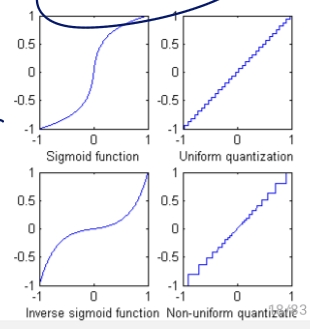
\includegraphics[width=0.5\linewidth,height=\textheight,keepaspectratio,alt={Various quantization scheme}]{capture_temp.jpg}
\caption{Various quantization scheme}
\end{figure}

\paragraph{HDR}\label{hdr}

High Dynamic Range (HDR) is a technology where we have various luminance
on the screen giving really good contrast in dark and bright area.
Usually, we combine multiple photos with various gains and then
recombine it all together with the various exposure.

\subsection{Sampling}\label{sampling}

\subsubsection{Integrate brightness over the cell
window}\label{integrate-brightness-over-the-cell-window}

\begin{figure}
\centering
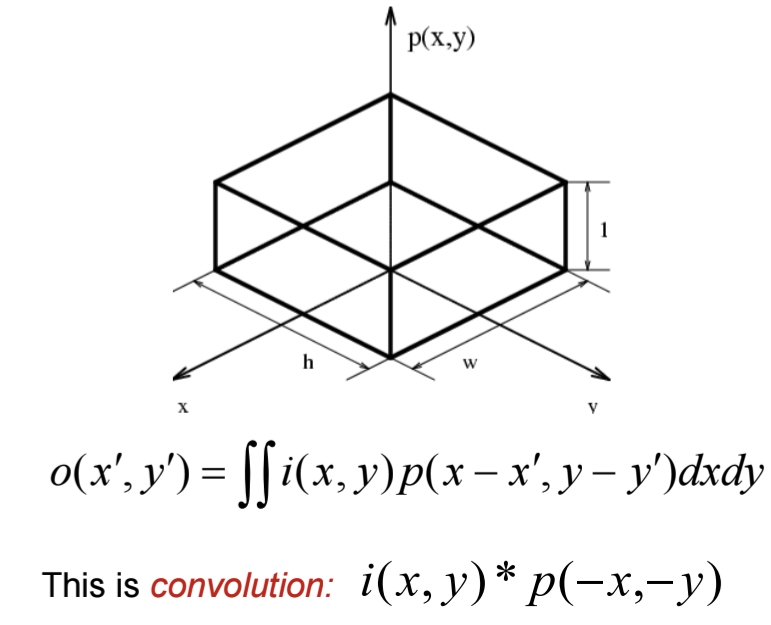
\includegraphics[width=0.5\linewidth,height=\textheight,keepaspectratio,alt={Integrating over a pixel cell}]{capture_temp-1.jpg}
\caption{Integrating over a pixel cell}
\end{figure}

This forms a convolution. Convolution are \textbf{linear},
\(f_1 \rightarrow g_1 \quad f_2 \rightarrow g_2 \Rightarrow af_1 + bf_2 \rightarrow ag_1+bg_2\)
, and \textbf{shift-invariant},
\(f(x,y) \rightarrow g(x,y) \Rightarrow f(x-a, y-b) \rightarrow g(x-a, y-b)\).

Convolutions are also commutative and associative as proven in the
Fourier domain.

\[
\mathfrak{F}(u) = \int_{-\infty}^{\infty} f(t) e^{-2i\pi x u}dx
\]

For the 2D case, we have \(e^{-2i\pi (ux + vy)}\) which has for Euler
form \(\cos(2\pi (ux+vy)) +  i\sin(2\pi (ux+vy))\). Now, the \(u\) and
\(v\) represents the frequency along the x and y dimensions. To obtain
the \(\lambda\) of the signal we need to take the norm of the frequency
for both axis inverted:

\[
\lambda = \frac{1}{\sqrt{u^2+v^2}}
\]

As in 1D, we can do Fourier transform to decomposition the image in a
bunch of frequencies. As in 1D, we have a complex results where the
magnitude is
\(|\mathfrak{F}(u,v)| = \sqrt{\mathbb{R}(\mathfrak{F}(u,v))^2 + \mathbb{I}(\mathfrak{F}(u,v))^2}\)
and the phase angle
\(\angle\mathfrak{F}(u,v) = \arctan(\mathbb{I}(\mathfrak{F}(u,v))/\mathbb{R}(\mathfrak{F}(u,v)))\).

\[
\mathfrak{F}(u,v) = \int_{-\infty}^{\infty}  \int_{-\infty}^{\infty} f(x,y) e^{-2i\pi (xu + yv)}dxdy
\]

\begin{figure}
\centering

\includegraphics[width=0.5\linewidth,height=\textheight,keepaspectratio,alt={Fourier decomposition of images}]{image-18.png}
\caption{Fourier decomposition of images}
\end{figure}

\begin{figure}
\centering

\includegraphics[width=0.5\linewidth,height=\textheight,keepaspectratio,alt={Repetitive patterns in an image creates repetitions in frequency domain}]{image-19.png}
\caption{Repetitive patterns in an image creates repetitions in
frequency domain}
\end{figure}

Removing patterns peak in frequency allows to remove periodic
background.

\begin{figure}
\centering

\includegraphics[width=0.5\linewidth,height=\textheight,keepaspectratio,alt={Mixmatch of phase and magnitude}]{image-20.png}
\caption{Mixmatch of phase and magnitude}
\end{figure}

\paragraph{Properties of spatial-frequency
domain}\label{properties-of-spatial-frequency-domain}

\begin{longtable}[]{@{}
  >{\raggedright\arraybackslash}p{(\linewidth - 2\tabcolsep) * \real{0.1842}}
  >{\raggedleft\arraybackslash}p{(\linewidth - 2\tabcolsep) * \real{0.8158}}@{}}
\toprule\noalign{}
\begin{minipage}[b]{\linewidth}\raggedright
Spatial domain
\end{minipage} & \begin{minipage}[b]{\linewidth}\raggedleft
Frequency domain
\end{minipage} \\
\midrule\noalign{}
\endhead
\bottomrule\noalign{}
\endlastfoot
Real & Real part \(\rightarrow\) even; Imaginary part \(\rightarrow\)
odd \\
Real,even & Real, even (cosine) \\
Real,odd & Imaginary, odd (sine) \\
\end{longtable}

Important to remember that a convolution in spatial domain is a
multiplication in the frequency domain and vice versa.

\begin{figure}
\centering

\includegraphics[width=0.5\linewidth,height=\textheight,keepaspectratio,alt={FFT approach}]{image-21.png}
\caption{FFT approach}
\end{figure}

We have the base image (the dot) and the the transfer function, MTF R,
which contains the amplification and phase shift information to every
frequency in the input image I.

\paragraph{Integrating with the
convolution}\label{integrating-with-the-convolution}

Re-using the integration over a cell window:

\[
o(x',y') = \int\int i(x,y)p(x-x', y-y') dxdy \leftrightarrow i(x,y) \ast p(-x,-y)
\]

We can then transform this \(p(x,y)\) round-point (as seen in the
previous figure) in a \(P(u,v)\)

\begin{align}
    P(u,v) &= \int_{-\infty}^{\infty} e^{-i 2 \pi (ux+vy)} p(x,y) dxdy\\
    &= wh \left( \frac{\sin(\pi wu)}{\pi wu} \right) \underbrace{\left( \frac{\sin (\pi h v)}{\pi hv} \right)}_{\text{sinc}}
\end{align}

The sinc function is predominantly low-pass \textbf{and} non-causal (no
phase shift) and it has phase reversal.

\subsection{Aliasing}\label{aliasing}

This corresponds to a 2D Dirac train convolution on the grid like:

\[
f(a,b) = \int\int f(x,y) \delta(x-a, y-b) dxdy
\]

The multiplication with the 2D pulse train with a spacing of distance w
and h:

\begin{align}
    &\sum_{k=-\infty}^\infty\sum_{l=-\infty}^\infty \delta(x-kw, y-lh)\\
    &\longleftrightarrow \frac{1}{wh}\sum_{k=-\infty}^\infty\sum_{l=-\infty}^\infty \delta(x-k\frac{1}{w}, y-l\frac{1}{h})
\end{align}

\begin{figure}
\centering

\includegraphics[width=0.5\linewidth,height=\textheight,keepaspectratio,alt={Basic sampling theorem}]{image-22.png}
\caption{Basic sampling theorem}
\end{figure}

Also, we need to do a Discrete Fourier Transform, DFT, to discretize the
space and frequency. We can also use FFT to bring the complexity of the
algorithm from \(N^2\) to \(N\log_2 N\).

\begin{align}
    &\sum_{m=0}^{M-1}\sum_{n=0}^{N-1} F(k,l) e^{2\pi i \left( \frac{km}{M} + \frac{ln}{N} \right)}\\
    &\longleftrightarrow F(k,l)= \frac{1}{MN} \sum_{m=0}^{M-1}\sum_{n=0}^{N-1} f(m,n) e^{-2\pi i \left( \frac{km}{M} + \frac{ln}{N} \right)}
\end{align}

\begin{figure}
\centering

\includegraphics[width=0.5\linewidth,height=\textheight,keepaspectratio,alt={Periodicity assumed in both domains, might introduce false high frequencies at image boundaries}]{image-23.png}
\caption{Periodicity assumed in both domains, might introduce false high
frequencies at image boundaries}
\end{figure}

\begin{figure}
\centering

\includegraphics[width=0.5\linewidth,height=\textheight,keepaspectratio,alt={We can have false high frequencies due to sampling}]{image-24.png}
\caption{We can have false high frequencies due to sampling}
\end{figure}

\begin{figure}
\centering

\includegraphics[width=0.5\linewidth,height=\textheight,keepaspectratio,alt={Solution on periodicity}]{image-25.png}
\caption{Solution on periodicity}
\end{figure}

Again, the Shannon theorem is important in 2D as well such that the
sampling distance \(w,h\) along the \(x,y\) axis must follow:

\[
w \leqslant \frac{1}{2 u_b} \qquad h \leqslant \frac{1}{2v_b}
\]

\section{Enhancement and feature
detection}\label{enhancement-and-feature-detection}

Strong from the knowledge of the previous section, we can do some
spectral filtering. For example, if we have some white noise in an image
we could apply a low pass filter on it to already remove a big part of
the noise while losing a marginal part of the actual picture
information. Usually, this will sorts of blur the image because sharp
edges are like high-frequency information.

\subsection{Enhancement - better look of
image}\label{enhancement---better-look-of-image}

Typically, HDR is a form of enhancement for better contrast. A cheaper
way of doing HDR is doing histogram equalisation which allows for better
usage of the full dynamic range available (a bit like gamma correction I
think).

\subsubsection{Histogram Equalisation}\label{histogram-equalisation}

This will makes the image more vibrant if we exploit more of the dynamic
range, we \textbf{redistribute} the intensities through a
\textbf{mapping that keeps their relative order}. Ideally, we make the
histogram \textbf{flat}.

\begin{figure}
\centering

\includegraphics[width=0.5\linewidth,height=\textheight,keepaspectratio,alt={We tune the Cumulative Intensity Probability - or CPD to a flat line}]{image-27.png}
\caption{We tune the Cumulative Intensity Probability - or CPD to a flat
line}
\end{figure}

We will compress the flat parts of the CPD, and expand the steepest one.
But the main issue, since we move bins, we want have a flat histogram,
we will just spread the bins more equally due to the \textbf{discrete
nature} of the input. On top, neigboring pixels won't always have the
same difference of intensities after the remapping (less problematic
though).

\subsubsection{Deblurring or Unsharp
masking}\label{deblurring-or-unsharp-masking}

If we deblur we actually increase the image sharpness. It's
\emph{simple, linear, image independent and effective}.

\begin{figure}
\centering

\includegraphics[width=0.5\linewidth,height=\textheight,keepaspectratio,alt={Imagine a vertical cut of image where x-axis is the pixel number and y-axis the grey-level}]{image-28.png}
\caption{Imagine a vertical cut of image where x-axis is the pixel
number and y-axis the grey-level}
\end{figure}

We see that we, indeed, make the edge steeper. Moreover, the difference
between the original-smooth makes a good fit for second order
derivative. This is a bit like running a diffusion process backwards.

The little over and under-shoots at the edge even magnifies the contrast
(Mach band effect).

\subsubsection{Inverse Filtering}\label{inverse-filtering}

Now, we shift gears and go into the frequency. We have the frequency
function that blurs the image with \(B(u,v)\). To undo it we apply
\(B'(u,v)\) such that \(B'(u,v)B(u,v) = 1\). Two danger here:

\begin{enumerate}
\def\labelenumi{\arabic{enumi}.}
\tightlist
\item
  What happens for \(B(u,v) = 0\)

  \begin{itemize}
  \tightlist
  \item
    Use a constant at the denominator --\textgreater{} Spurious
    high-frequencies :'(
  \item
    \(B'(u,v)=B(u,v)/(B(u,v)^2 + C)\) --\textgreater{} Much better !
    Wiener-like reduces C for larger SNR and vice versa.
  \end{itemize}
\item
  For low \(B(u,v)\) after noise was applied --\textgreater{} may
  over-fit the noise\ldots{}
\end{enumerate}

\subsubsection{Noise Suppression}\label{noise-suppression}

\paragraph{Low pass}\label{low-pass}

As introduced, we can use a low-pass filter for noise suppression. The
main problem with applying this rectangular (actually a circle) window
is the rippling due to the sinc function as seen here

\begin{figure}
\centering

\includegraphics[width=0.5\linewidth,height=\textheight,keepaspectratio,alt={Rippling effect}]{image-29.png}
\caption{Rippling effect}
\end{figure}

\subsection{Features - edge and corner
detections}\label{features---edge-and-corner-detections}

\textbf{ABOVE SHOULD BE THE START OF CHAPTER ABOUT ENHANCEMENT AND
EDGES}

P.41

\paragraph{Convolution filters}\label{convolution-filters}

It is based on the insight that noise affects high frequencies the most
due to their low SNR. To build a low-pass filter, we will use an
averaging kernel such:

\[
\begin{pmatrix}
    1 & 1 & 1\\
    1 & 1 & 1\\
    1 & 1 & 1
\end{pmatrix} = \underbrace{\begin{pmatrix}
    1 & 1 & 1
\end{pmatrix} \ast \begin{pmatrix}
    1\\
    1\\
    1\\
\end{pmatrix}}_{\text{separable filter}}
\]

The two \((1,1,1)\) vectors can be seen in the \emph{frequency} domain
as \(1 + 2\cos(2\pi u)\) for the horizontal domain or
\(1 + 2\cos(2\pi v)\) in the vertical one. The intuition for this is to
look at the vector as a 1D image centered around the middle value.
Finally, the convolution can be simplified in the frequency domain as:

\[
(1 + 2\cos(2\pi u))(1 + 2\cos(2\pi v))
\]

\begin{figure}
\centering

\includegraphics[width=0.5\linewidth,height=\textheight,keepaspectratio,alt={Representation in 3D of the function}]{image-26.png}
\caption{Representation in 3D of the function}
\end{figure}

The function is purely real and low-pass with some phase reversal! We
can again derivate something similar for a 5x5 kernel:

\[
(1 + 2\cos(2\pi u) + 2\cos(4\pi u))(1 + 2\cos(2\pi v) + 2\cos(4\pi v))
\]

With this one, the phase reversal is even more significant, the higher
the frequency the more it looks like a sinc function. This creates more
ripples and disturbing effects. Hard to get no ripple and a real
low-pass for higher order functions.

From all those experiments we can draw 3 conclusions:

\begin{enumerate}
\def\labelenumi{\arabic{enumi}.}
\tightlist
\item
  Separable filters can be implement more efficiently
\item
  Better to go in the frequency domain for large kernel
\item
  Keep it simple, mask of boolean or power of 2 are cheap!
\end{enumerate}

\subsubsection{Binomial filters}\label{binomial-filters}

They are here to solve the ripple and low-pass issue of the convolution
filters presented before. This guarantees no phase reversal.

\[
\begin{pmatrix}
    1 & 2 & 1\\
    2 & 4 & 2\\
    1 & 2 & 1
\end{pmatrix} = \begin{pmatrix}
    1 & 2 & 1
\end{pmatrix} \ast \begin{pmatrix}
    1\\
    2\\
    1\\
\end{pmatrix} \longleftrightarrow (2 + 2\cos(2\pi u))(2 + 2\cos(2\pi v))
\]


\includegraphics[width=0.5\linewidth,height=\textheight,keepaspectratio,alt={Gaussian filters are limit case of binomial filters}]{image-27.png}\{width=50\%\}

Note that noise removal linear filters will exhibit blurring due the
fact they cannot difference noise and actual information.

\subsubsection{Median}\label{median}

Instead of averaging over using a kernel of ones, we take the median -
the middle point of neighborhood of pixel. We don't create a new grey
level, we take the one in the middle.

\begin{figure}
\centering

\includegraphics[width=0.5\linewidth,height=\textheight,keepaspectratio,alt={Median filters principle - credits: southampton.ac.uk}]{image-28.png}
\caption{Median filters principle - credits: southampton.ac.uk}
\end{figure}

One advantage of a median filter is the fact it is robust against
outliers and it will preserve the contrast instead of smooching out all
the values and making the image more blurry.

\begin{itemize}
\tightlist
\item
  Discard outliers
\item
  Preserve discontinuities
\end{itemize}

But, it will loose in details (especially small areas). Moreover, give a
patchy effect instead of a smooth uniform color.

\subsubsection{Anisotropic filters - all-in-on of
filtering}\label{anisotropic-filters---all-in-on-of-filtering}

This filter does:

\begin{enumerate}
\def\labelenumi{\arabic{enumi}.}
\tightlist
\item
  Binomial smoothing between edges
\item
  Unsharp masking at edges
\end{enumerate}

For this, we need to cover edge detection

\begin{longtable}[]{@{}
  >{\raggedright\arraybackslash}p{(\linewidth - 4\tabcolsep) * \real{0.1982}}
  >{\centering\arraybackslash}p{(\linewidth - 4\tabcolsep) * \real{0.7297}}
  >{\centering\arraybackslash}p{(\linewidth - 4\tabcolsep) * \real{0.0721}}@{}}
\caption{Summary table of the enhancement procedures}\tabularnewline
\toprule\noalign{}
\begin{minipage}[b]{\linewidth}\raggedright
Operation name
\end{minipage} & \begin{minipage}[b]{\linewidth}\centering
Description
\end{minipage} & \begin{minipage}[b]{\linewidth}\centering
Linear ?
\end{minipage} \\
\midrule\noalign{}
\endfirsthead
\toprule\noalign{}
\begin{minipage}[b]{\linewidth}\raggedright
Operation name
\end{minipage} & \begin{minipage}[b]{\linewidth}\centering
Description
\end{minipage} & \begin{minipage}[b]{\linewidth}\centering
Linear ?
\end{minipage} \\
\midrule\noalign{}
\endhead
\bottomrule\noalign{}
\endlastfoot
Histogram equalisation & Re-sort histogram to create a more linear
Cumulative Probability Density & V \\
Unsharp mask & & V \\
Inverse Filtering & Realize the opposite operation. Need to carefully
handle low SNR with a constant. & V \\
Low pass & Removes noise since it affects more high-frequencies due to
low SNR & V \\
Binomial & Like low-pass but avoids phase reversal & V \\
Median & Take the middle point instead of the mean & X \\
Anisotropic & Binomial between edges - Unsharp at edge & X \\
\end{longtable}

\subsection{Enhancement and Feature
Detection}\label{enhancement-and-feature-detection-1}

\subsubsection{Edges}\label{edges}

\begin{quote}
\textbf{Definition:}

Edge correspond to image locations with strong intensity changes due to:

\begin{enumerate}
\def\labelenumi{\arabic{enumi}.}
\tightlist
\item
  Reflectance
\item
  Orientation of shape normals (its surface) - the object's edge
\item
  Illuminations (shadow)
\end{enumerate}

The hardest challenge in edge detection is linking up all the pixels
into a good line drawing.
\end{quote}

The methods cover here will be based on the gradient which gives the
direction of the steepest change along as its magnitude being the rate
of change:

\[
\text{gradient } = \left( \frac{\partial f}{\partial x}, \frac{\partial f}{\partial y} \right) \qquad \text{magnitude } = \sqrt{\left( \frac{\partial f}{\partial x}\right)^2 + \left( \frac{\partial f}{\partial y} \right)^2}
\]

2 methods will be covered using \textbf{isotropic} operators\footnote{there
  exists other (and better) operators but too complex for this class}:

\begin{enumerate}
\def\labelenumi{\arabic{enumi}.}
\tightlist
\item
  Locating high intensity gradient magnitude
\item
  Locating inflection points in the intensity profiles
\end{enumerate}

\begin{figure}
\centering

\includegraphics[width=0.5\linewidth,height=\textheight,keepaspectratio,alt={With curvature being a sort of second order derivative}]{image-29.png}
\caption{With curvature being a sort of second order derivative}
\end{figure}

\subsubsection{Gradient}\label{gradient}

The idea is to:

\begin{enumerate}
\def\labelenumi{\arabic{enumi}.}
\tightlist
\item
  measure the gradient \textbf{magnitude} of all the steep slopes in the
  image. This operator is isotropic since there are equal contribution
  of the x and y direction.
\item
  Measure the angle \(\theta\) that maximizes
  \(\frac{\partial f}{\partial x'} = \frac{\partial f}{\partial x} \cos (\theta) + \frac{\partial f}{\partial y} \sin(\theta)\)
  this yields
  \(\theta_{xtr} = \tan^{-1}\left( \frac{\partial f}{\partial y} / \frac{\partial f}{\partial x} \right)\)
\end{enumerate}

The gradient is a non-linear operator of \(\partial / \partial x\) which
are linear, shift-invariant ! So this can be implemented using a
convolution, the \textbf{Sobel masks} which are separable and cheap to
implement. The Sobel masks are a bit like a binomial filter but with a
derivative in the middle. The idea is to have a strong response for high
frequencies (edges) and low response for low frequencies (flat areas).:

\[
\frac{\partial}{\partial x} = (-1,0,1) \ast (1,2,1)^\top = \begin{pmatrix}
    -1 & 0 & 1\\
    -2 & 0 & 2\\
    -1 & 0 & 1
\end{pmatrix} \qquad \frac{\partial}{\partial y} = \begin{pmatrix}
    -1 & -2 & -1\\
    0 & 0 & 0\\
    1 & 2 & 1
\end{pmatrix}
\]

From their outputs, we take the square root of the sum of their squares,
take the arctan which will give us the orientation of the edge!

Again we can move to the frequency domain where we remember we can see
the vector as a 1D image centered around the middle value. The Fourier
transform of the Sobel mask is:

\[
(-1,0,1) \longleftrightarrow 2i \sin(2\pi u) \qquad (1,2,1) \longleftrightarrow 2 + 2\cos(2\pi u)
\]

We see that it is pass band along the u-dir (red on the graph) and
low-pass along the v-dir (green on the graph).

\begin{figure}
\centering

\includegraphics[width=0.5\linewidth,height=\textheight,keepaspectratio,alt={Function in 3D}]{image-30.png}
\caption{Function in 3D}
\end{figure}

\begin{figure}
\centering

\includegraphics[width=0.5\linewidth,height=\textheight,keepaspectratio,alt={Combining the two (top left: x-dir, top right: y-dir)}]{image-31.png}
\caption{Combining the two (top left: x-dir, top right: y-dir)}
\end{figure}

It is a great technique to map individual pixel edges, but cannot be
perfect to edge detection. There can be gap, several pixels thick, weak
or salient edges, and so on. But Sobel masks are the optimal 3 x 3
convolution filters with integer coefficients for step edge detection.

\subsubsection{Zero-crossing}\label{zero-crossing}

First, we want to do edge thinning, to reduce a several pixel thick edge
to only one continguous line. Once we found the gradient, we want to
look at the direction giving the maximum gradient and interpolate to get
these values. We can also apply the hysteresis thresholding to link up
the edges. The idea is to have a high threshold for strong edges and a
low threshold for weak edges. We then link the weak edges to the strong
ones if they are connected.

\begin{figure}
\centering

\includegraphics[width=0.5\linewidth,height=\textheight,keepaspectratio,alt={Canny edges}]{image-32.png}
\caption{Canny edges}
\end{figure}

To do zero-crossing detection, we need to use second order derivative
and make it equal to 0 to find inflexion points. This is linear + shift
invariant (convolution) and isotropic (equal contribution of x and y).
The Laplacian is sensitive to noise, so we often add a smoothing step
(Gaussian) before applying the Laplacian. This is called the Laplacian
of Gaussian (LoG) operator.

\[
\nabla^2 f = \frac{\partial^2 f}{\partial x^2} + \frac{\partial^2 f}{\partial y^2} = 0
\]

We can also use the Difference of Gaussian (DoG) which is a good
approximation of the LoG and is much faster to compute. The idea is to
take the difference between two Gaussian blurred images with different
standard deviations.

\[
G_1 = \begin{pmatrix}
    0 & 1 &0 \\
    1 & -4 & 1\\
    0 & 1 & 0
\end{pmatrix} \qquad G_2 = \begin{pmatrix}
    1 & 2 & 1\\
    2 & -12 & 2\\
    1 & 2 & 1
\end{pmatrix}
\]

This DoG method will give us a closed-contour as it is based on the
second order derivative. The zero-crossing will give us the edge
location. The main issue is that it is not very good at linking up edges
and can be quite sensitive to noise.

\subsubsection{Harris corner detection}\label{harris-corner-detection}

This method will distinguish between homogeneous areas, edges and
corners. The idea is to look at the eigenvalues of the second moment
matrix of the gradient. If both eigenvalues are small, we have a
homogeneous area. If one eigenvalue is large and the other is small, we
have an edge. If both eigenvalues are large, we have a corner. The
second order moment matrix is given by:

\[
\begin{pmatrix}
    \left(\frac{\partial f}{\partial x}\right)^2 & \frac{\partial f}{\partial x} \frac{\partial f}{\partial y}\\
    \frac{\partial f}{\partial x} \frac{\partial f}{\partial y} & \left(\frac{\partial f}{\partial y}\right)^2
\end{pmatrix}
\]

\begin{figure}
\centering

\includegraphics[width=0.7\linewidth,height=\textheight,keepaspectratio,alt={Principle of Harris}]{image-33.png}
\caption{Principle of Harris}
\end{figure}

The idea is to find the directions of minimal and maximal change in the
image. We move the kernel by a small amount (u,v) where our \(w\) window
function can be either a box or a Gaussian. We then look at the change
in intensity which is given by:

\[
E(u,v) = \sum_{x,y} w(x,y) [f(x+u, y+v) - f(x,y)]^2
\]

\[
E(u,v) \approx [u,v] M \begin{bmatrix}
    u\\ v
    \end{bmatrix} \qquad \text{with } M = \sum_{x,y} w(x,y) \begin{pmatrix}
    \left(\frac{\partial f}{\partial x}\right)^2 & \frac{\partial f}{\partial x} \frac{\partial f}{\partial y}\\
    \frac{\partial f}{\partial x} \frac{\partial f}{\partial y} & \left(\frac{\partial f}{\partial y}\right)^2
\end{pmatrix}
\]

To analyze the harris detector, we use the iso-lines
\(= det -k trace^2 = \lambda_1 \lambda_2-k(\lambda_1 + \lambda_2)^2\).
Where \(\lambda_1\) and \(\lambda_2\) are the eigenvalues of the matrix
\(M\) and represent a change in one or the other direction. If the
iso-line is positive, we have a corner. If it is negative, we have an
edge. If it is zero, we have a homogeneous area. The main issue with
this method is that it is not very good at distinguishing between edges
and corners in the presence of noise.

\begin{figure}
\centering

\includegraphics[width=0.5\linewidth,height=\textheight,keepaspectratio,alt={Iso-lines for Harris}]{image-34.png}
\caption{Iso-lines for Harris}
\end{figure}

\section{Image decomposition}\label{image-decomposition}

Images can be projected in various orthogonal basis, (pixels, fourier
domain, \ldots). We can also do a rotation for example, but the most
important thing is that we use \textbf{unitary
transformations}\(\rightarrow U^\ast U = I\).

\subsection{PCA}\label{pca}

We want to reduce the dimensionality of the data while preserving as
much variance as possible. We can do this by projecting the data onto
the eigenvectors of the covariance matrix. The eigenvectors with the
largest eigenvalues will be the principal components. This is a linear
transformation that preserves the distances between points in the
original space. It is an \textbf{unitary transformation} but
\textbf{data dependent}. We want to reduce the dimension of the data
while keeping as much information as possible.

\begin{figure}
\centering

\includegraphics[width=0.5\linewidth,height=\textheight,keepaspectratio,alt={Central idea of PCA}]{image-35.png}
\caption{Central idea of PCA}
\end{figure}

The Shannon entropy \(H(x)\) quantifies the amount of entropy in a data
set with a distribution P. This fact is interesting, because most
pictures only span a sub-set of the total possible images. For example,
natural images have a lot of structure and regularity, which means that
they have a low entropy compared to random noise. This is why we can use
PCA to reduce the dimensionality of the data while preserving most of
the information.

\[
H(x) = -\sum_{i} P(x_i) \log P(x_i)
\]

This issue with the lack of spanning in high-dimensional space is often
referred to as the \textbf{curse of dimensionality}. PCA is a solution
to this problem. Some intuitive explanation: 1D:
\((r+\delta)/r \approx 1 + \delta/r\); 2D:
\((r+\delta)^2/r^2 \approx 1 + 2\delta/r\); D:
\((r+\delta)^D/r^D \approx 1 + D\delta/r\). So the volume of the space
grows exponentially with the dimension, which means that we need an
exponentially large number of samples to cover the space. PCA helps us
to reduce the dimensionality of the data while preserving most of the
information.

For the PCA, we use the Pearson correlation coefficient. We need to be
careful with it as it only indicates linear correlation between two
variables!

\[
p_{ij} = \frac{cov(x,y)}{\sigma_i \sigma_j} = \frac{\sum_{i=1}^N (x_i - \bar{x})(y_i - \bar{y})}{\sqrt{\sum_{i=1}^N (x_i - \bar{x})^2} \sqrt{\sum_{i=1}^N (y_i - \bar{y})^2}}
\]

We first find the highest component with the maximum of correlation,
then we find the second one with the lowest correlation. We can then
apply a rotation in a high dimensional space.

By working around the mean, we benefit from parserval-equality which
indicates the variances in \(x_i\) will be the same in \(z_j\). This
indicates a redistribution of the energy.

\[
\sum_{i=1}^p \sigma_i^2 = \sum_{j=1}^p \tilde{\sigma}_j^2
\]

\subsubsection{Method}\label{method}

With \(x\) a vector of \(p\) variables. We first look for a linear
combination \(c_1^\top x\) which has the maximum variance. We then look
for a second linear combination \(c_2^\top x\) which has the maximum
variance and is uncorrelated with the first one. We repeat this process
until we have \(p\) linear combinations. The first few linear
combinations will capture most of the variance in the data, which is why
we can reduce the dimensionality of the data by keeping only the first
few principal components.

By relying on the Gaussian distribution postulat, we can derive a
covariance matrix. Note, we need to center the data around the mean
first. We need to maximize so
\(var(c_1^\top x) = \sum c_1^\top x (c_1^\top x)^\top =c_1^\top \sum (xx^T) c_1 = c_1^\top C c_1\)
with \(C\) the covariance matrix. And we make sure that
\(c_1^\top c_1 =1\) to avoid trivial solution.

\begin{figure}
\centering

\includegraphics[width=0.5\linewidth,height=\textheight,keepaspectratio,alt={Covariance matrix}]{image-36.png}
\caption{Covariance matrix}
\end{figure}

We can then use the Lagrange multiplier with the constrained mentioned
ealier:

\[
\mathcal{L}(c_1, \lambda) = c_1^\top C c_1 - \lambda (c_1^\top c_1 - 1)
\]

\[
\frac{\partial \mathcal{L}(c_1, \lambda)}{\partial c_1} = 2C c_1 - 2\lambda c_1 =  2c_1 \underbrace{(C- \lambda I)}_{\text{eingevalue problem}} = 0 \qquad \frac{\partial \mathcal{L}(c_1,\lambda)}{\partial \lambda} = c_1^\top c_1 - 1 = 0
\]

So
\(c_1^\top C c_i = c_1^\top \lambda c_1 = \lambda c_1^\top c_1 = \lambda\)
with \(\lambda\) as large as possible. Decorrelation and orthogonality
are the same thing in this case since we are in a Euclidean space. So
\(c_2^\top C c_1 = c_2^\top \lambda c_1 = \lambda c_2^\top c_1 = 0\).

\begin{figure}
\centering

\includegraphics[width=0.5\linewidth,height=\textheight,keepaspectratio,alt={Proof of orthogonality between c\_1 and c\_2}]{image-37.png}
\caption{Proof of orthogonality between \(c_1\) and \(c_2\)}
\end{figure}

We can again use a Lagrange multiplier to ensure decorrelation:

\begin{figure}
\centering

\includegraphics[width=0.5\linewidth,height=\textheight,keepaspectratio,alt={Decorrelation}]{image-38.png}
\caption{Decorrelation}
\end{figure}

\begin{figure}
\centering

\includegraphics[width=0.5\linewidth,height=\textheight,keepaspectratio,alt={Important remark}]{image-39.png}
\caption{Important remark}
\end{figure}

\subsubsection{Usage}\label{usage}

\begin{itemize}
\tightlist
\item
  Classification of crops: using Near-infrared, Red, Green data. We see
  some correlation between red and green + near-infrared. We can
  compress the data to roughly 60\% while retaining similar performance.
\item
  Culture and heritage: reveal details that wasn't visible before.
  Quickly find the most important features in the data.
\item
  Image compression: same density in neihboring pixels. Issue is that
  image of N pixels =\(N^2\) base. So \(N^2*N^2\) for the covariance
  matrix. PCA allows us to reduce the dimensionality of the data while
  preserving most of the information. We can then use a lossy
  compression algorithm to further reduce the size of the data.

  \begin{itemize}
  \tightlist
  \item
    We can use the \textbf{eingenfaces} of the covariance matrix as a
    basis for the image. We can then project the image onto this basis
    and keep only the first few components to reduce the size of the
    data. This is called \textbf{eigenface} method. We form a human face
    base using a base of already existing faces. (do not forget to
    substract the mean !)
  \end{itemize}
\end{itemize}

\subsubsection{Limitations}\label{limitations}

As described before, the Pearson correlation coefficient is only for
linear correlation. Moreover, the PCA is based on the assumption of a
Gaussian distribution.

A solution is the Interesting Component analysis where we find multiple
``interesting'' components. Or we can use the Linear Discriminant
Analysis (LDA) which is a supervised method that finds the linear
combination of features that best separates two or more classes of
objects or events. It is based on the idea of maximizing the
between-class variance while minimizing the within-class variance. This
approach is better for non Gaussian distribution.

There is also the support vector machine which look at an hyper plane to
find the best separation between classes.

PCA looks like the Harris corner detector but a few things chenge:

\begin{itemize}
\tightlist
\item
  No substraction by mean in Harris
\item
  No normalization in Harris
\end{itemize}

\section{Surface features color and
texture}\label{surface-features-color-and-texture}

\subsection{Color}\label{color}

It is important to distinguish between two important spectre of the
color:

\begin{enumerate}
\def\labelenumi{\arabic{enumi}.}
\tightlist
\item
  Radiometry: physical measurement of the light (radiance, irradiance,
  reflectance, \ldots)
\item
  Photometry: how the human eye perceives the light (brightness, colour,
  \ldots)
\end{enumerate}

A light \(l\) with a spectral composition \(c(\lambda)\) and the human
that perceives it with a sensitivity \(h(\lambda)\), with the constant
\(k = 683\) lm/W. Ofc, we can span only the human visible spectrum which
is roughly between 400 and 700 nm. The perceived brightness is then
given by the following equation:

\[
l = k \int_{\lambda=0}^\infty c(\lambda) h(\lambda) d\lambda
\]

Human perception of color can be summarized with Brightness, Huhe, and
saturation.

\begin{figure}
\centering

\includegraphics[width=0.5\linewidth,height=\textheight,keepaspectratio,alt={Retinal cones of a human; occupancy S:5-10, M:30, L:60}]{image-41.png}
\caption{Retinal cones of a human; occupancy S:5-10, M:30, L:60}
\end{figure}

So the human has 3 sensitivity curves and not just one from the equation
aforementioned. We have 3 responses for the full spectrum. So if 2
sources are observed with the same response for the 3 cones, they will
be perceived as the same color. This is called \textbf{metamerism}.

\subsubsection{Commission Internationale de l'Éclairage
(CIE)}\label{commission-internationale-de-luxe9clairage-cie}

They standartized the color space with 3 primaries:

\begin{enumerate}
\def\labelenumi{\arabic{enumi}.}
\tightlist
\item
  Red: 700 nm
\item
  Green: 546.1 nm
\item
  Blue: 435.8 nm
\end{enumerate}

With this, we can match \(m_j\) a source \(C(\lambda)\) with a
combination of the 3 primaries \(P_j(\lambda)\) such that:

\[
C(\lambda) = \sum_{j=1}^3 m_j P_j(\lambda)
\]

We can derive the following:

\[
    R_i(C) = \int \sum_{j=1}^3 m_j P_j(\lambda) H_i(\lambda) d\lambda = \sum_{j=1}^3  m_j \underbrace{\int  P_j(\lambda) H_i(\lambda)}_{l_{i,j}\text{ Sensitivity of a primary can be determined offline}} d\lambda
\]

This makes a really simple system of 3 linear equations for the human
eye. If we use different primaries \(L'\), we can find a new set of
coefficients \(m'\) such that:

\[
\sum_{j=1}^3 m_j l_{i,j} = Ri\qquad LM = R \qquad L'M' = R \quad m' = L'^{-1}Lm
\]

\paragraph{Tristimulus value}\label{tristimulus-value}

As white is the combination of all the colors, we can use the white
point as a reference for the color. We can then define the tristimulus
value as:

\[
T_j = \frac{m_j}{w_j} \qquad T_1 = T_1= T_3 = 1 \quad \text{for white}
\]

\begin{figure}
\centering

\includegraphics[width=0.5\linewidth,height=\textheight,keepaspectratio,alt={Spectral matching curves}]{image-42.png}
\caption{Spectral matching curves}
\end{figure}

We notice negative colors which cannot be produced by a combination of
the primaries. This is a problem for the display of colors. Moreover,
for some colors, a triple of primaries cannot represent it! However the
tristimulus values still contain brightness information, we can
normalize to only get chromatic information:

\[
t_j = \frac{T_j}{\sum_{j=1}^3 T_j} \qquad t_1 + t_2 + t_3 = 1
\]

So now, 2 chromaticity coordinates are enough to represent the color
(saturation and hue). This forms the XYZ coordinates of the CIE, with X
being a mix of red/green cones, the Y the luminance and Z blue light
primarly. The mapping matrix is

\[
\begin{pmatrix}
    X\\
    Y\\
    Z
\end{pmatrix} = \begin{pmatrix}
    0.490 & 0.310 & 0.200\\
    0.177 & 0.813 & 0.011\\
    0.000 & 0.010 & 0.990
\end{pmatrix}\begin{pmatrix}
    R\\
    G\\
    B
\end{pmatrix}
\]

\begin{figure}
\centering
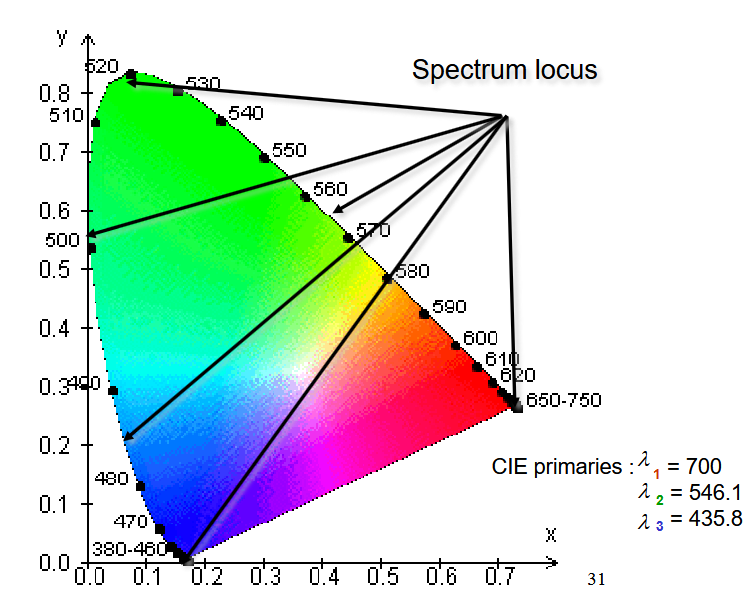
\includegraphics[width=0.5\linewidth,height=\textheight,keepaspectratio,alt={CIE color triangle}]{image-43.png}
\caption{CIE color triangle}
\end{figure}

Inside this triangle, the mix of two colors in some quantities lie on
the straight line between those two colors.

Screen standard tries to span as much as this CIE triangle to have the
highest fidelity possible. Such color coordinates need 3 primaries on
the CIE triangle + the central white point --\textgreater{} 4 points.
Also the projection is skewed on the triangle, much more information lie
in the bottom blue corner and red corner than in the top green one.

The CIE u-v is a solution which represents area more faithfully.

\[
u = \frac{4x}{-2x+12y+3} \qquad v = \frac{6y}{-2x+12y+3}
\]

\subsubsection{Constancy}\label{constancy}

Many optical illusions exists where our brain is tricked and interprets
colors when there are none or the context can influences our perception.
We often interpret the ambient light to infer the result of the dot
product on our human cones. This is called the \textbf{color constancy}.
The brain is trying to infer the color of the object by taking into
account the ambient light. This is why we can see a white paper as white
even if it is under a red light.

\subsection{Texture}\label{texture}

Many textures exist such as oriented vs isotropic, stochastic vs
regular, coarse vs fine, \ldots{}

\subsubsection{Fourier features}\label{fourier-features}

We analyze the texture based on the power spectrum of the Fourier
transform. A peak in the power spectrum indicates a strong periodicity
in the image. The orientation of the peak indicates the orientation of
the texture. The width of the peak indicates the coarseness of the
texture. The more spread out the peak is, the more stochastic the
texture is.

One problem with this method is the fact that is captures the global
periodicity of the image but not the local one. Moreover, it is not very
good at capturing the orientation of the texture. Finally, it is not
very good at capturing the coarseness of the texture.

\[
\int \int |F(u,v)|^2 du dv
\]

\begin{figure}
\centering
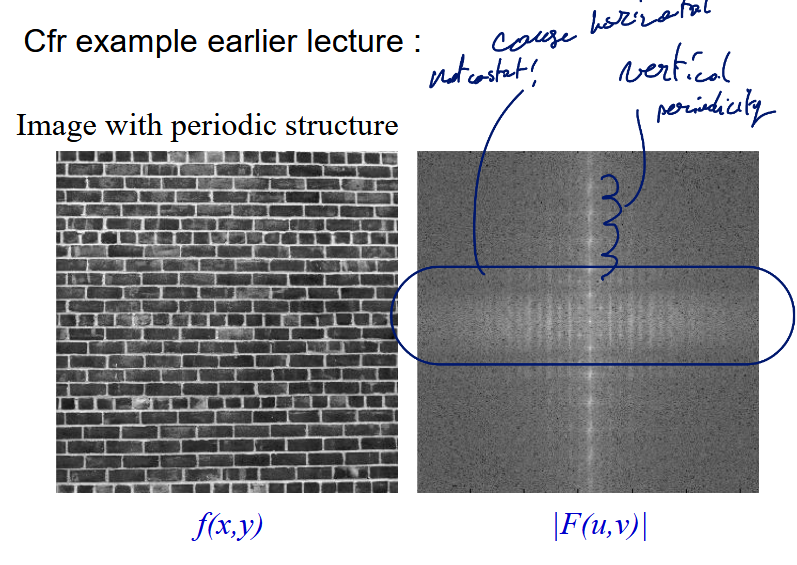
\includegraphics[width=0.5\linewidth,height=\textheight,keepaspectratio,alt={Periodicity}]{image-44.png}
\caption{Periodicity}
\end{figure}

\subsubsection{Cooccurrence matrices}\label{cooccurrence-matrices}

It is inspired by the histogram idea, but this time we will take a
chosen offset between two points and count how many i,j pair exists in a
double entry matrix. This will give us a measure of the texture based on
the co-occurrence of pixel values. We can then derive some statistics
from this matrix such as contrast, homogeneity, energy, \ldots{}

\begin{figure}
\centering
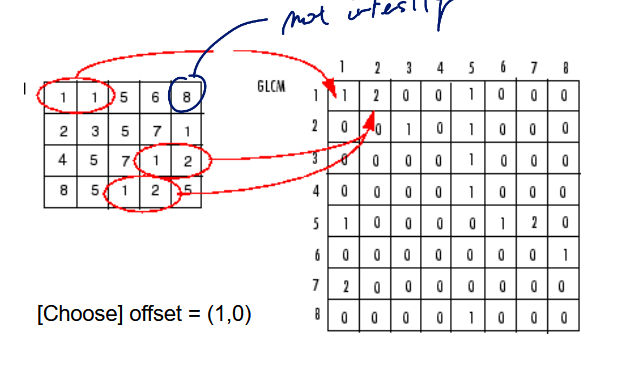
\includegraphics[width=0.5\linewidth,height=\textheight,keepaspectratio,alt={Cooccurrence matrix}]{image-45.png}
\caption{Cooccurrence matrix}
\end{figure}

\begin{longtable}[]{@{}
  >{\raggedright\arraybackslash}p{(\linewidth - 2\tabcolsep) * \real{0.2353}}
  >{\raggedright\arraybackslash}p{(\linewidth - 2\tabcolsep) * \real{0.7647}}@{}}
\caption{Summary table of the features derived from the cooccurrence
matrix}\tabularnewline
\toprule\noalign{}
\begin{minipage}[b]{\linewidth}\raggedright
Feature
\end{minipage} & \begin{minipage}[b]{\linewidth}\raggedright
Expression
\end{minipage} \\
\midrule\noalign{}
\endfirsthead
\toprule\noalign{}
\begin{minipage}[b]{\linewidth}\raggedright
Feature
\end{minipage} & \begin{minipage}[b]{\linewidth}\raggedright
Expression
\end{minipage} \\
\midrule\noalign{}
\endhead
\bottomrule\noalign{}
\endlastfoot
Contrast & \(\sum_{i,j} (i-j)^2 C(i,j)\) \\
Homogeneity & \(\sum_{i,j} \frac{1}{1+          \| i-j \| } C(i,j)\) \\
Energy & \(\sum_{i,j} C(i,j)^2\) \\
Entropy & \(-\sum_{i,j} C(i,j) \log C(i,j)\) \\
Max. Probability & \(\max_{i,j} C(i,j)\) \\
\end{longtable}

\subsubsection{Filter banks}\label{filter-banks}

\paragraph{Laws}\label{laws}

\begin{figure}
\centering
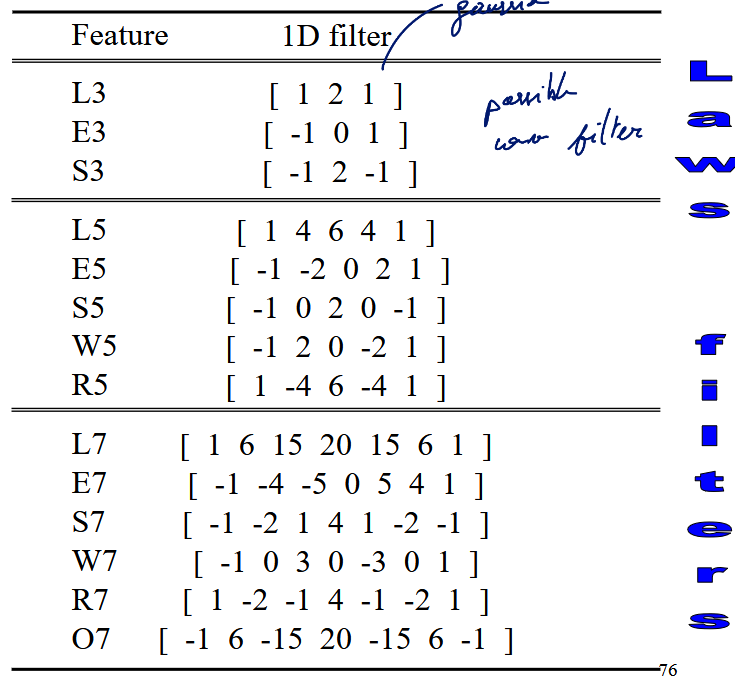
\includegraphics[width=0.5\linewidth,height=\textheight,keepaspectratio,alt={Laws filter}]{image-46.png}
\caption{Laws filter}
\end{figure}

We can start from 1D laws filter to form more advanced decomposed 2D
filters. L=Level, E=Edge, S=Spot, W=Wave, R=Ripple. The idea is to have
a set of filters that can capture different types of textures. For
example, the L5E5 filter will capture edges, while the E5L5 filter will
capture spots. We can then apply these filters to the image and analyze
the response to get a measure of the texture. It is simle but really
effective. Detection or classification nby assigning features /
statistical metrics to the outputs.

\paragraph{Gabor}\label{gabor}

It is a gaussian envelope modulated by a sinusoidal plane wave. It is a
band-pass filter that can capture both the frequency and orientation of
the texture. We can tweak the sensitivity and directionality of the
filter. The Gabor filter is defined as:

\[
g(x,y) = \exp\left( -\frac{x^2 + \gamma^2 y^2}{4\Delta_{x,y}^2} \right) \cos\left( 2\pi u^\ast x + \phi \right) \longleftrightarrow G(u,v) = \frac{1}{4\pi\Delta_{u,v}^2}\exp\left( -\frac{(u-u^\ast)^2 +  v^2}{4\Delta_{u,v}^2} \right) + \exp\left( -\frac{(u+u^\ast)^2 +  v^2}{4\Delta_{u,v}^2} \right)
\]

\begin{figure}
\centering
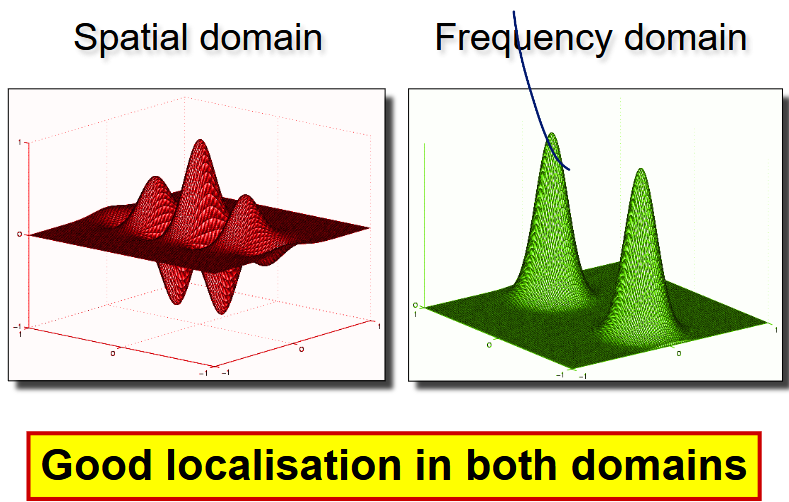
\includegraphics[width=0.5\linewidth,height=\textheight,keepaspectratio,alt={Gabor filters}]{image-47.png}
\caption{Gabor filters}
\end{figure}

\paragraph{Eigenfilters}\label{eigenfilters}

\begin{enumerate}
\def\labelenumi{\arabic{enumi}.}
\tightlist
\item
  Create a mask to be shifted over a training image
\item
  Within the mask, collect intensity statistics
\item
  PCA --\textgreater{} eigenvectors --\textgreater{} eigenfilters
\item
  Determine energies of eigenfilters of eigenfilter outputs
\end{enumerate}

We often need large but sparse filters for good efficacy. Can be great
for damage inspection or QA in industry.

We often need to use multiple eigenfilters to capture different aspects
of the texture. A great technique to compile multiple eingefilters
together and quickly locate error or irregularities in the texture is
the \textbf{Manhalanobis distance of the energies}:

\begin{align}
    D_M(x,y) = \sqrt{(r(x,y)-\mu)^\top \Sigma^{-1}(r(x,y) - \mu)}\\
    \mu = \frac{1}{N} \sum_{i=1}^N r(x_i,y_i)\qquad \Sigma = diag(\lambda_1, \lambda_2, ..., \lambda_K)
\end{align}

Mahalanobis distance DM measures how unusual this combination of
responses is compared to normal texture. A response along a very stable
direction (small eigenvalue) counts more. A response along a highly
variable direction (large eigenvalue) is less surprising.

\section{Motion Extraction}\label{motion-extraction}

Many animals are dependent on motion detection to outperform camouflage.
Only with a few dots in motion can infer many informations.

\subsection{Definition}\label{definition}

\subsubsection{Optical flow}\label{optical-flow}

\begin{quote}
Optical flow

Apparent motion of brightness patterns in the image. Ideally it is the
the projection of the 3D motion vectors of the image
\end{quote}

\begin{quote}
Motion Field

3D motion of the scene as seen through the camera. It is the projection
of the 3D motion vectors of the scene onto the image plane.
\end{quote}

We can use 2D vectors to depict the translation of the pixels forming
the optical flow. Motion field != optical flow (e.g., the barbershop
pole turning around horizontally but it looks like it's sliding
vertically, same for a perfect sphere with an uniform texture, it will
look stable even if it starts spinning)

The goal with optical flow is to measure for each pixel between two
frames where each went. It is a non-trivial task and requires a few
assumptions to be achievable:

\begin{enumerate}
\def\labelenumi{\arabic{enumi}.}
\tightlist
\item
  Same brightness
\item
  Minimal motion
\end{enumerate}

\paragraph{Mathematics}\label{mathematics}

With \(I(x,y,t)\) the intensity of the pixel at position (x,y) at time
t, we can measure the difference with:

\[
I(x,y,t) = I(x+\delta x, y+\delta y, t+\delta t)\qquad \frac{dI}{dt} = \underbrace{\frac{\partial I}{\partial x}}_{I_x} \underbrace{\frac{dx}{dt}}_{u} + \underbrace{\frac{\partial I}{\partial y}}_{I_y} \underbrace{\frac{dy}{dt}}_{vD} + \underbrace{\frac{\partial I}{\partial t}}_{I_t} = 0
\]

This equation states that if one were to track the image projections of
a scene point through the video, it would not change its intensity. This
tends to be true over short lapses of time.

Note that \(dI/dt\) represents the change of intensity when following a
physical point through the images; but \(\partial I/\partial t\) is the
change of intensity at a fixed location in the image. The difference
between these two is the motion of the point in the image.

\begin{figure}
\centering
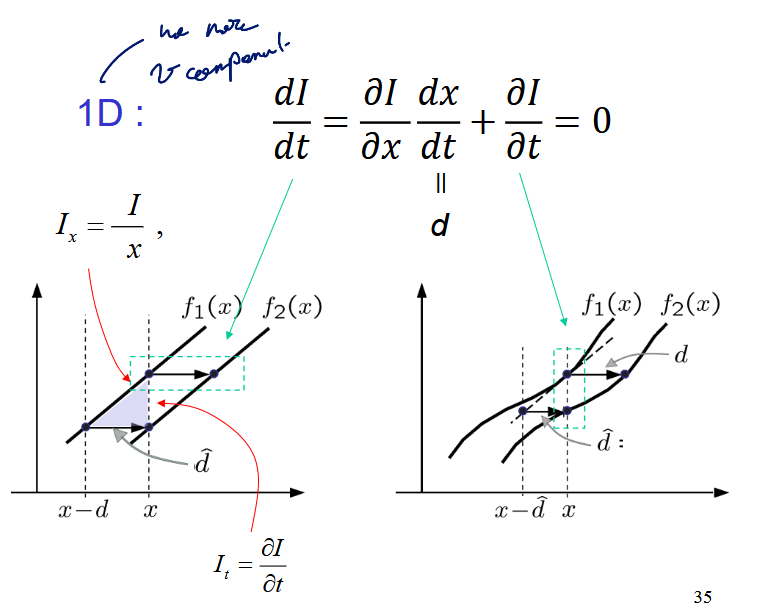
\includegraphics[width=0.5\linewidth,height=\textheight,keepaspectratio,alt={Optical flow in 1D}]{image-48.png}
\caption{Optical flow in 1D}
\end{figure}

The issue with this equation is that \(I_x\),\(I_y\), and \(I_t\) can be
measured. However, \(u\) and \(v\) are unknwon, 1 equation 2 unknowns =
\textbf{Aperture Problem}.

\begin{figure}
\centering
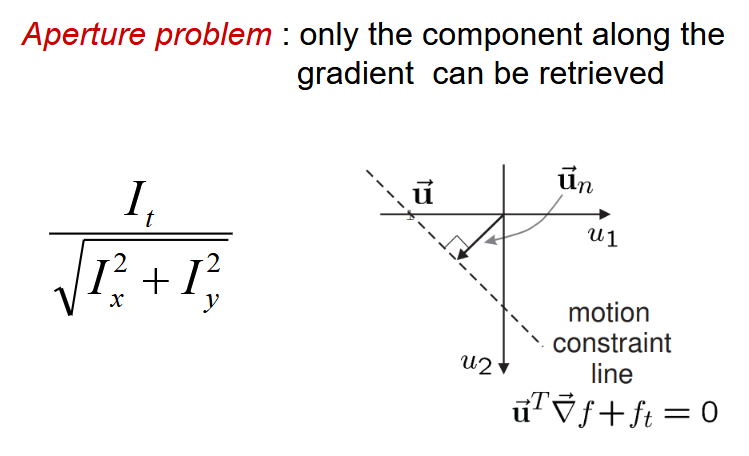
\includegraphics[width=0.5\linewidth,height=\textheight,keepaspectratio,alt={Aperture problem}]{image-49.png}
\caption{Aperture problem}
\end{figure}

We only zoom in one tiny part of the frame and thus we miss the overall
motion by only looking at such details. The problem can be solved with:

\begin{enumerate}
\def\labelenumi{\arabic{enumi}.}
\tightlist
\item
  Higher derivative of intensity --\textgreater{} expensive + noisy
\item
  For planar intensity profile, problem cannot be solved (higher order
  derivative are zero)
\end{enumerate}

\subsection{Horn \& Schunk}\label{horn-schunk}

Additional smoothness constraint is added to the equation to solve the
aperture problem. The idea is to minimize the following energy function:

\[
e_S = \int \int ((u_x^2 + u_y^2 + v_x^2 + v_y^2) dx dy) \qquad e_C = \int \int (I_x u + I_y v + I_t)^2 dx dy \qquad \text{minimize } e = e_S + \lambda e_C
\]

We need to find a function that extremize the functionals (functions
that takes vector in and scalar out)

\begin{figure}
\centering
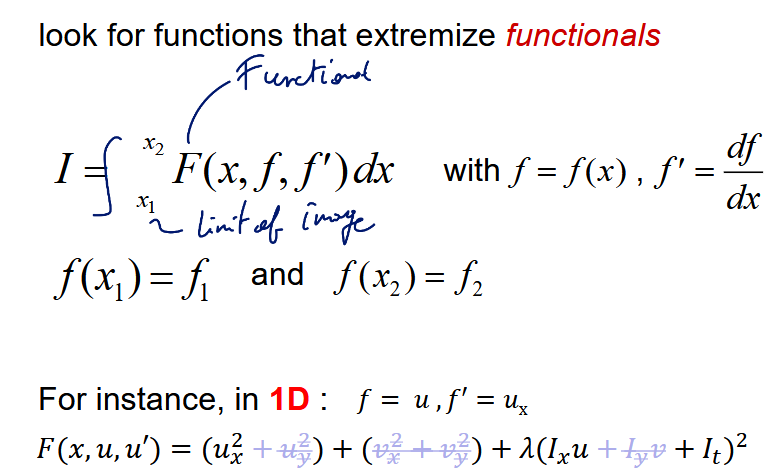
\includegraphics[width=0.5\linewidth,height=\textheight,keepaspectratio,alt={1D example of our functional}]{image-50.png}
\caption{1D example of our functional}
\end{figure}

\begin{figure}
\centering
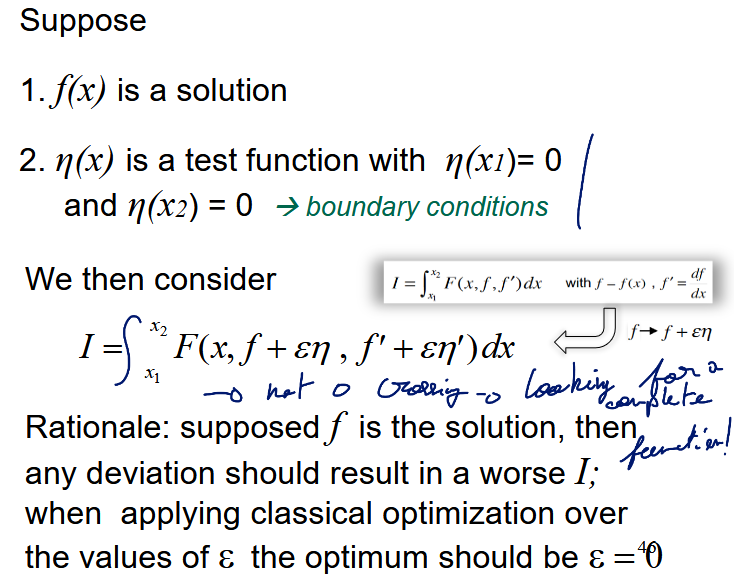
\includegraphics[width=0.5\linewidth,height=\textheight,keepaspectratio,alt={Calculus of variation}]{image-51.png}
\caption{Calculus of variation}
\end{figure}

This allows to reformulate an optimization over a function into an
optimization over a scalar. We can use
\(dI/d\varepsilon|_{\varepsilon=0} =0\). We can use Euler-Lagrange
equation to find the function that extremize the functional.

\textbf{TODO: PAGES 49 - 62} --\textgreater{} Take time to understand

\begin{enumerate}
\def\labelenumi{\arabic{enumi}.}
\tightlist
\item
  We use regularization, need sometimes to pose extra constraints
\item
  Errors at object boundaries, smoothness constraint no longer valid
\end{enumerate}

\subsection{Lucas \& Kanade}\label{lucas-kanade}

It uses the same optical flow equation but used an area based
regression. We assume that the flow is constant in a small neighborhood
of the pixel under consideration (local optimization). We can then solve
for the flow vector using least squares. The idea is to minimize the
following energy function:

\begin{align}
    A &= \begin{bmatrix}
        I_x(q_1) & I_y(q_1)\\
        I_x(q_2) & I_y(q_2)\\
        \vdots & \vdots\\
        I_x(q_n) & I_y(q_n)
    \end{bmatrix} & v&= \begin{bmatrix}
        V_x\\ V_y
    \end{bmatrix} & b&=\begin{bmatrix}
        -I_t(q_1)\\
        -I_t(q_2)\\
        \vdots\\
        -I_t(q_n)
    \end{bmatrix}
\end{align}

\[
A^\top A v = A^\top b \qquad v = (A^\top A)^{-1} A^\top b
\]

\[
\begin{bmatrix}
    V_x\\
    V_y
\end{bmatrix} = \begin{bmatrix}
    \sum_{i=1}^n I_x(q_i)^2 & \sum_{i=1}^n I_x(q_i) I_y(q_i)\\
    \sum_{i=1}^n I_x(q_i) I_y(q_i) & \sum_{i=1}^n I_y(q_i)^2
\end{bmatrix}^{-1} \begin{bmatrix}
    -\sum_{i=1}^n I_x(q_i) I_t(q_i)\\
    -\sum_{i=1}^n I_y(q_i) I_t(q_i)
\end{bmatrix}
\]

It cannot always reliably calculate the flow, apperture problem, it
requires a lot of texture in all direction to be reliable. So, to detect
interesting points, we often use the Harris-detector to find interesting
spots and apply area based flow around each key point. This is called
the \textbf{feature tracking}. However, it does not respect Taylor
expansion.

Another technique is to use a form of coarse to fine to estimate the
flow even better with various size.

\subsection{Active contours}\label{active-contours}

The idea is to track a contour from one key frame to another one. It is
like an elastic band we adjust frame by frame. It is a good and robust
approach for noise especially whan we know what object we are tracking
(e.g., lips).

\begin{figure}
\centering
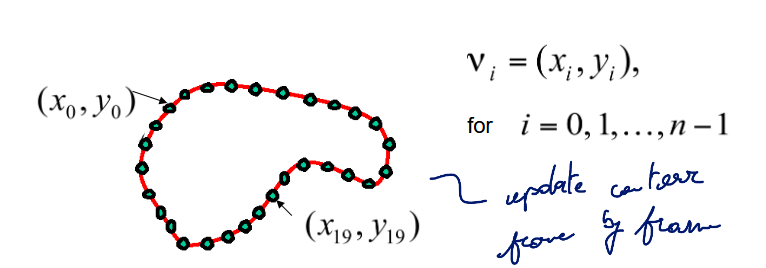
\includegraphics[width=0.5\linewidth,height=\textheight,keepaspectratio,alt={Active contours}]{image-52.png}
\caption{Active contours}
\end{figure}

We use some discrete representation of the contour which is a list of 2D
points (vertices). We define an energy function that we want to
minimize. The energy function is a combination of an internal energy
that depends on the shape of the contour (known shape, \ldots) and an
external energy that depends on the image (edges present in the image,
attracts the contour to the edges of the image). The internal energy is
given by:

\[
E_{total} = E_{internal} + E_{external} 
\]

\paragraph{External}\label{external}

Energy for a point of a curve and the whole curve:

\[
E_{external}(v) = -(|G_x(v)|^2 + |G_y(v)|^2) \qquad E_{external} = -\sum_{i=0}^{n-1} (|G_x(x_i,y_i)|^2 + |G_y(x_i,y_i)|^2)
\]

\paragraph{Internal}\label{internal}

We use the elasticity and the bending energy to define the internal
energy. The elasticity energy is given by:

\[
E_{internal}(v(s)) = \underbrace{\alpha \left| \frac{dv}{ds} \right|^2}_{\text{elasticity}} + \underbrace{\beta \left| \frac{d^2 v}{ds^2} \right|^2}_{\text{bending}}
\]

For our discrete representation, we can use finite differences to
approximate the derivatives:

\[
\frac{dv}{ds} \approx v_{i+1} - v_i \qquad \frac{d^2 v}{ds^2} \approx (v_{i+1} - v_i) - (v_i - v_{i-1}) = v_{i+1} - 2v_i + v_{i-1}
\]

Internal energy for the whole curve

\[
E_{internal} = \sum_{i=0}^{n-1} \left( \alpha |v_{i+1} - v_i|^2 + \beta |v_{i+1} - 2v_i + v_{i-1}|^2 \right)
\]

For the elastic energy, we often a term \(d\) to avoid that the energy
collapse on itself and so we take the initial distance \(d\).

We can also use a term to penalize the length of the curve to avoid that
it grows indefinitely. This is called the balloon energy.

\begin{figure}
\centering
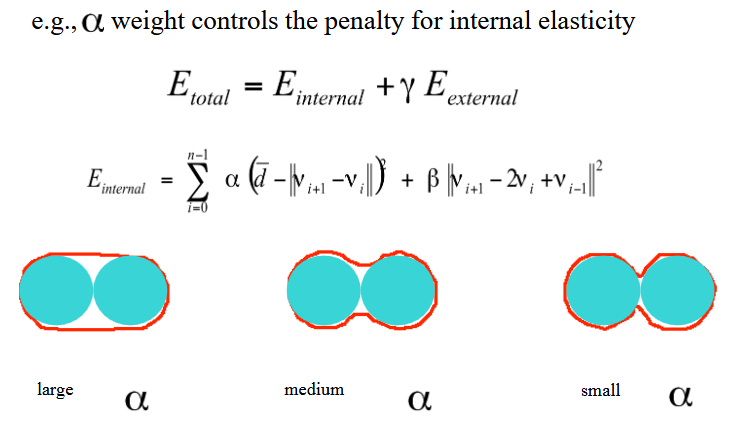
\includegraphics[width=0.5\linewidth,height=\textheight,keepaspectratio,alt={Active contours}]{image-53.png}
\caption{Active contours}
\end{figure}

\subsubsection{Energy minimization}\label{energy-minimization}

\paragraph{Greedy}\label{greedy}

For each point we simply look where we can move them to minimize the
energy. Usually small window (5x5) around the point. It is simple but
can get stuck in local minima and requires decent initialization.

\paragraph{Dynamic programming}\label{dynamic-programming}

Use a form of the viterbi algorithm to propagate down the energy and
find the optimal path. It is more robust to local minima but can be
computationally expensive.

\paragraph{Gradient Vector flow (GVF)}\label{gradient-vector-flow-gvf}

\begin{figure}
\centering
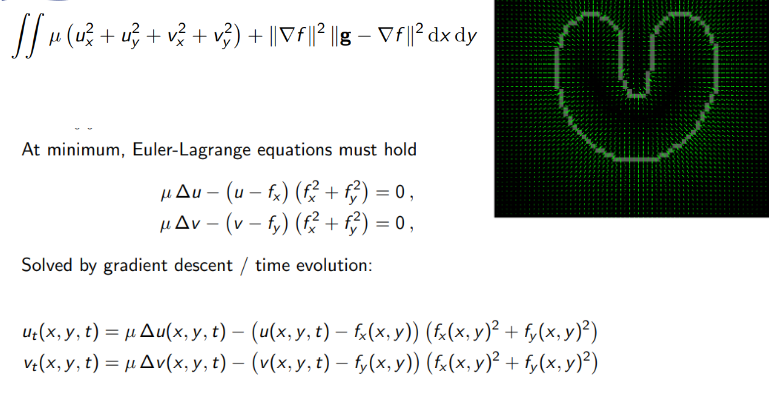
\includegraphics[width=0.5\linewidth,height=\textheight,keepaspectratio,alt={GVF (Informational only)}]{image-54.png}
\caption{GVF (Informational only)}
\end{figure}

\begin{figure}
\centering
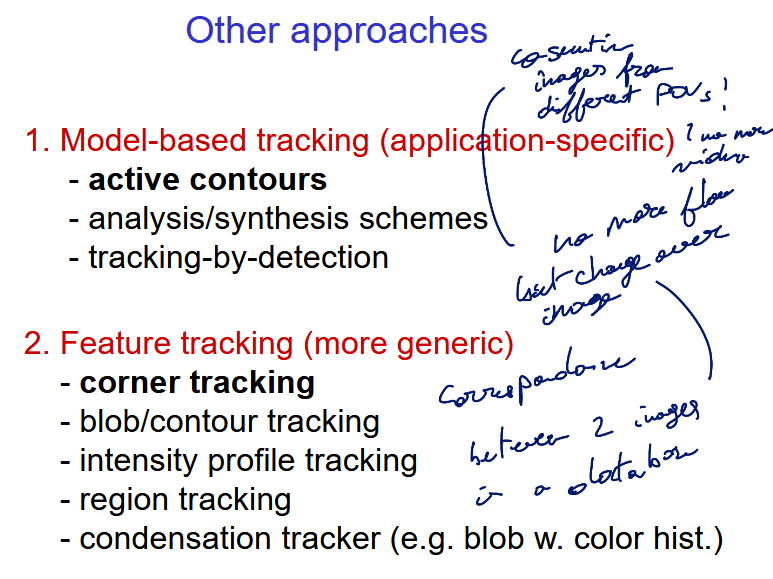
\includegraphics[width=0.5\linewidth,height=\textheight,keepaspectratio,alt={Other approaches}]{image-55.png}
\caption{Other approaches}
\end{figure}

\section{Local features \& Feature
matching}\label{local-features-feature-matching}

The goal is to recognize landmarks accross pictures, or faces, \ldots{}
It is based on previous knowledge heavily inspired from Sobel, Harris
Laplacians, Lucas Kanade (for feature tracking), \ldots{} All of this
wil help us build SIFT.

We want to find local features but it is not trivial as scales will be
problematic in this task. But achieving it will enable 3D
reconstruction, recognition of objects, image matching, image retrieval,
\ldots{} For this we rely on 3 main components:

\begin{enumerate}
\def\labelenumi{\arabic{enumi}.}
\tightlist
\item
  Detection: of the important landmark and interest points
\item
  Description: of the local features around the interest points (feature
  vector)
\item
  Matching: of the features between different images
\end{enumerate}

We want our detector to be:

\begin{itemize}
\tightlist
\item
  repeatable: be consistent
\item
  distinctive: highlight good interest points. Moreover it should
  precisely match each interest point
\item
  invariant: no matter the scale or the rotation, we should be able to
  find the same interest points (geomtric or photometric changes). Keep
  deriving the same feature points trhoughout the images (otherwise
  impossible to match them)
\item
  compact / efficient: realtime applications, embedded systems, \ldots{}
  with limited compute power, use binary feature descriptors
\item
  find local interest points: the smaller, the less likely it will be
  affected by occlusion, deformation, \ldots{} we can approximate local
  surfaces using local planes
\end{itemize}

Everything will be a tradeoff between these different properties. For
example, we can have a very distinctive feature that is not very
repeatable, or a very repeatable feature that is not very distinctive.
We need to find the right balance between these properties for our
specific application.

\subsection{Detection}\label{detection}

\subsubsection{Rotation invariant
detectors}\label{rotation-invariant-detectors}

\paragraph{Harris corner points}\label{harris-corner-points}

We can use the harris detector to detect interesting feature points such
as corners. When selecting the point, the window encapsulating it should
make it recognizable and if we slide around we should witness a large
change in intensity. M is symmetric since we have change in both
direction (corner) and we have

\[
M = \Sigma \begin{bmatrix}
    I_x^2 & I_xI_y\\
    I_xI_y & I_y^2
\end{bmatrix} = \begin{bmatrix}
    \lambda_1 & 0\\
    0 & \lambda_2
\end{bmatrix} \qquad Mx_i = \lambda_i x_i \qquad R(x,y) = det(M) - \alpha tr(M)^2 = \lambda_1 \lambda_2 - \alpha(\lambda_1 + \lambda_2)^2
\]

We get the R scores for each image window, find points where surrounding
window gave high R, finally take the points of local maxima of R.

\begin{figure}
\centering
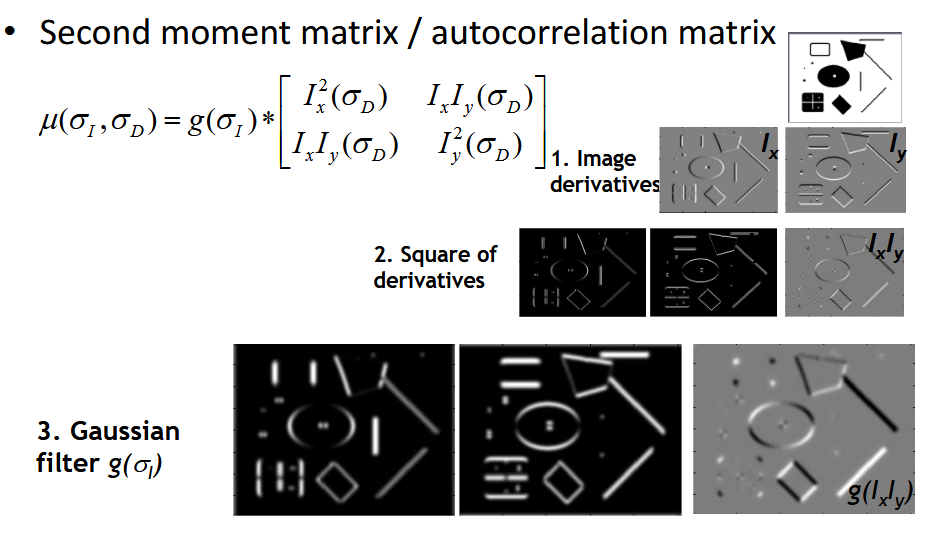
\includegraphics[width=0.5\linewidth,height=\textheight,keepaspectratio,alt={Harris detector in practice}]{image-56.png}
\caption{Harris detector in practice}
\end{figure}

We develop a ``cornerness'' function where both eigenvalues are large
(high det).

\[
har = \det[\mu(\sigma_I,\sigma_D)] - \alpha \cdot \text{trace}[\mu(\sigma_I,\sigma_D)] = g(I^2_x) g(I^2_y) - g(I_x I_y)^2 - \alpha (g(I^2_x) + g(I^2_y))^2
\]

It is rotation invariant \(M =X\Sigma X^{-1}\) with \(X\) the rotation
matrix. However, it is not scale invariant as the size of the window
will change with the scale. Moreover, it is not very good at detecting
corners in low contrast images.

\paragraph{Laplacian of Gaussians}\label{laplacian-of-gaussians}

Laplacian of Gaussians (LoG) is a second order derivative operator that
is used to detect edges and corners in images. It is defined as the
convolution of the image with a Gaussian kernel followed by the
Laplacian operator. The idea is to find the zero-crossings of the LoG
response, which correspond to edges and corners in the image. It is
rotation invariant but not scale invariant as the size of the Gaussian
kernel will change with the scale.

Important to match the size of the kernel to have an optimum detection.

\subsubsection{Scale invariant
detectors}\label{scale-invariant-detectors}

\paragraph{Multi-scale approach}\label{multi-scale-approach}

We can use the Harris or LoG where we will try multiple size of kernel.
We can then look for local maxima in the scale space. This is called the
\textbf{scale-space representation}. The idea is to create a pyramid of
images with different scales and look for local maxima in this pyramid.
This is a simple but effective way to achieve scale invariance.

It is important to use a scale-normalized derivatives to achieve scale
invariance. This is done by multiplying the derivatives by a factor of
\(\sigma^n\) where \(n\) is the order of the derivative and \(\sigma\)
is the scale. This way, the response of the detector will be the same
regardless of the scale.

\paragraph{Local extrema in scale
space}\label{local-extrema-in-scale-space}

We find the two highest response and then try to match them together. We
can then look for local maxima in the scale space to find the interest
points. This is called the \textbf{scale-space extrema}. The idea is to
find the points that are local maxima in both space and scale. This is a
more robust way to find interest points as it takes into account the
scale of the features.

\begin{figure}
\centering
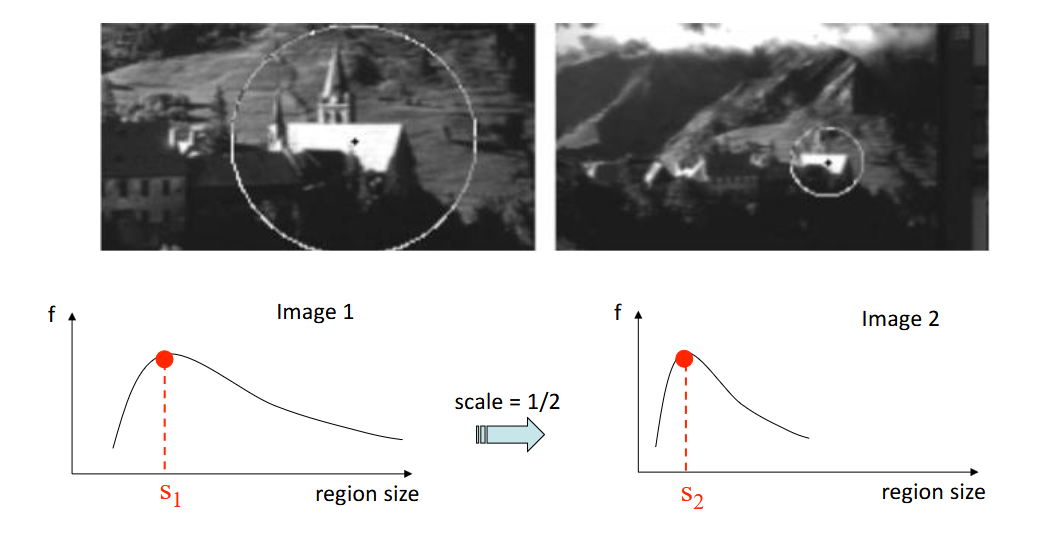
\includegraphics[width=0.5\linewidth,height=\textheight,keepaspectratio,alt={Visual explanation}]{image-57.png}
\caption{Visual explanation}
\end{figure}

\subsubsection{Affine invariant
detectors}\label{affine-invariant-detectors}

The idea is to take advantage of regular human-made plane structure to
inverse the affine transformation through projective transformation:
\textbf{homography}. We can then apply the Harris or LoG detector on the
rectified image to find the interest points. This is called the
\textbf{affine-invariant detectors}. The idea is to find the points that
are invariant to affine transformations. This is a more robust way to
find interest points as it takes into account the affine transformations
that can occur in the image. For local features, this behavior is less
important.

\paragraph{MSER}\label{mser}

\begin{figure}
\centering
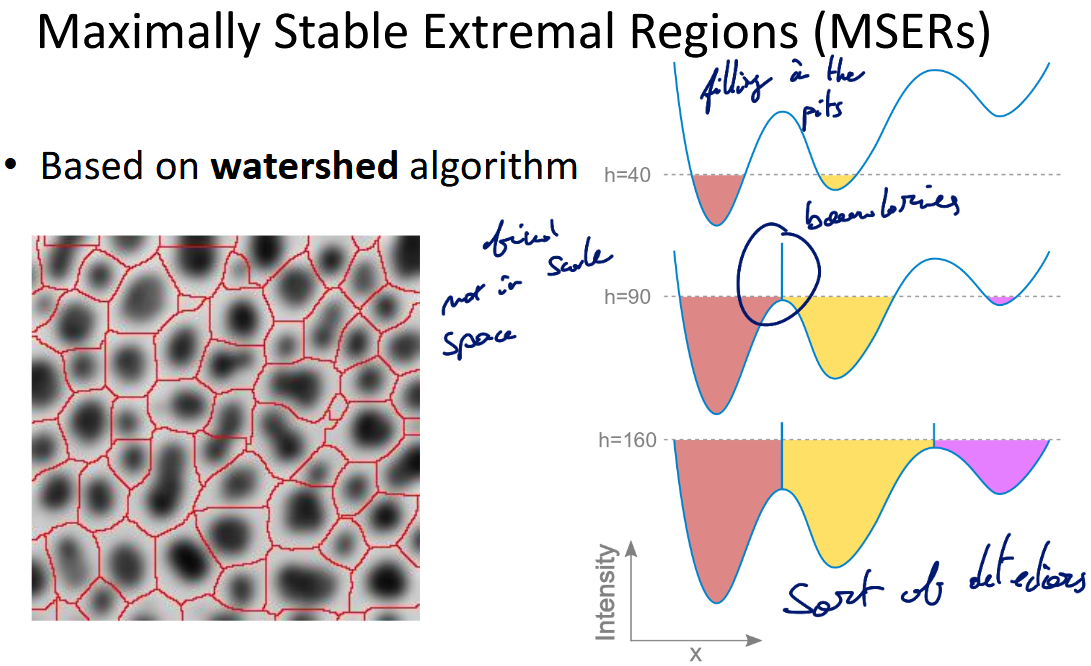
\includegraphics[width=0.5\linewidth,height=\textheight,keepaspectratio,alt={Maximally Stable Extremal Regions}]{image-58.png}
\caption{Maximally Stable Extremal Regions}
\end{figure}

We ``flood'' the area until the change in area is too large. We can then
look for local maxima in the scale space to find the interest points.
This is called the \textbf{maximally stable extremal regions (MSER)}.
The idea is to find the points that are local maxima in both space and
scale.

Another improvement, we can use ellipsoid instead of weird grainy
boundaries, this makes matching easier.

\subsection{Description}\label{description}

\subsubsection{Scale Invariant Feature Transform
(SIFT)}\label{scale-invariant-feature-transform-sift}

Handle changes in viewpoint up to about 60 degree out of plane rotation.
Can also handle changes in illumination, partial occlusion, \ldots{} We
want to find a descriptor that is invariant to these changes. We can use
the local image patch around the interest point to create a descriptor.
The idea is to create a histogram of oriented gradients (HOG) around the
interest point. This is called the \textbf{SIFT descriptor}. It has two
steps: rotation normalization and then descriptor computation.

\paragraph{1. Rotation normalization}\label{rotation-normalization}

\begin{itemize}
\tightlist
\item
  take window around detected interest point (\(3\sigma\))
\item
  Compute edge orientation (gradient angle - 90) for each pixel
\item
  Histogram of edge orientation with 36 bins (10 degree each)

  \begin{itemize}
  \tightlist
  \item
    Weight by grad magnitude, bilinear interpolation, distance to
    center, \ldots{}

    \begin{itemize}
    \tightlist
    \item
      bilinear interpolation: to find an unkonw point in a 2D space
      located inside a square. We take the 4 points of the square and we
      weight them by the area covered between the point and the unknown.
      The closer the point is, the more weight it has. This allows us to
      have a smooth transition between the bins of the histogram.
    \end{itemize}
  \end{itemize}
\item
  Find the dominant rotation and rotate the patch to make it horizontal
  pointing to the right.
\end{itemize}

\begin{figure}
\centering
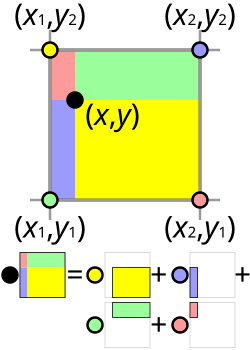
\includegraphics[width=0.25\linewidth,height=\textheight,keepaspectratio,alt={Bilinear interpolation (wikipedia)}]{image-59.png}
\caption{Bilinear interpolation (wikipedia)}
\end{figure}

\paragraph{2. Descriptor computation}\label{descriptor-computation}

\begin{itemize}
\tightlist
\item
  Divide the square patch into 4x4 sub-regions
\item
  For each sub-region, compute a histogram of edge orientation with 8
  bins (45 degree each)

  \begin{itemize}
  \tightlist
  \item
    16*8 = 128 dimensions for the descriptor
  \end{itemize}
\item
  Normalize the descriptor to have unit length to achieve invariance to
  changes in illumination.
\end{itemize}

It is a robust descriptor because of the use of histograms, bilinear
weighting, smoothing with gaussian kernel. However it is not invairant
to affine transformations, it is not very good at handling changes in
scale, and it is not very good at handling changes in viewpoint. It is
good for small geometric transformations and robust for photometric
changes.

We often combine the SIFT descriptor with other method or even CNN.

\subsection{Matching}\label{matching}

As the name implies, the goal is to determine correspondences between
features in different images. We can use the Euclidean distance between
the descriptors to find the closest match. Another approach is the
\textbf{Sum of Squared Differences (SSD)}.

However, this can lead to many false matches. To avoid this, we can use
a ratio test where we compare the distance of the closest match to the
distance of the second closest match. If the ratio is below a certain
threshold, we consider it a good match. This is called the
\textbf{Lowe's ratio test}.

In general we take one feature in an image and use a defined distance
function to test all the features in the second and find the minimum
distance.

\section{3D Acquisition}\label{d-acquisition}

\begin{figure}
\centering
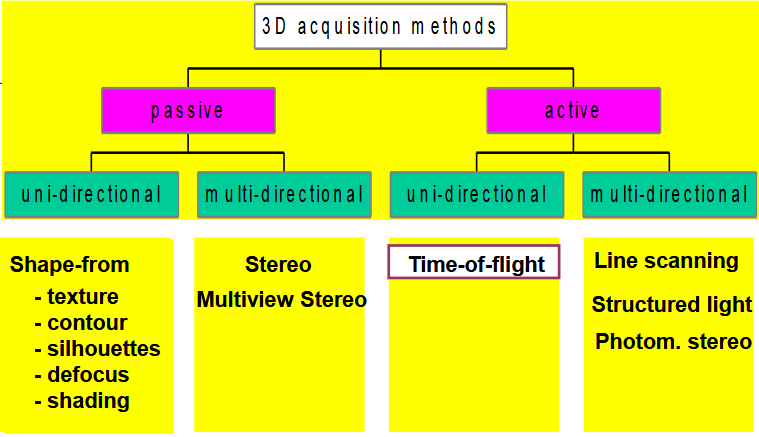
\includegraphics[width=0.5\linewidth,height=\textheight,keepaspectratio,alt={Map of the chapter}]{image-65.png}
\caption{Map of the chapter}
\end{figure}

\subsection{Passive: no interaction with the
scene}\label{passive-no-interaction-with-the-scene}

\subsubsection{Uni-directional}\label{uni-directional}

\paragraph{Shape from texture}\label{shape-from-texture}

By using a repetitive pattern (e.g.~checkerboard) it is possible to
infer the 3D structure of the scene by looking at the orientation of the
surface. If an isotropic pattern creates an anisotropic image
statistics, we can invert this operation.

\paragraph{Shape from contour}\label{shape-from-contour}

We make assumption about the contour shape, we can use the symmetry of
an object to infer its 3D structure. For example, if we see a circle in
the image, we can infer that it is a sphere in 3D. If we see an ellipse,
we can infer that it is an ellipsoid in 3D. We can also use the
compactness to infer the 3D structure.

\paragraph{Shape from silhouette}\label{shape-from-silhouette}

By using multiple points of view, we can create a voxel in 3D to
reconstruct in 3D the object.

\paragraph{Shape from defocus}\label{shape-from-defocus}

To infer depth in a picture, we look at the sharpness of the image at
various zoom focus to reconstruct the 3D scene. We can create alpha map
with this technique.

\paragraph{Shape from shading}\label{shape-from-shading}

We can use directional lightning (often known direction) to evaluate the
depth of the image. By using the Lambertian assumption (reflection
depend on an angle; a surface scatters incoming light uniformly in all
directions, equally bright in all direction, ideal matte material), we
can find correspondance using reflectance maps.

\begin{figure}
\centering
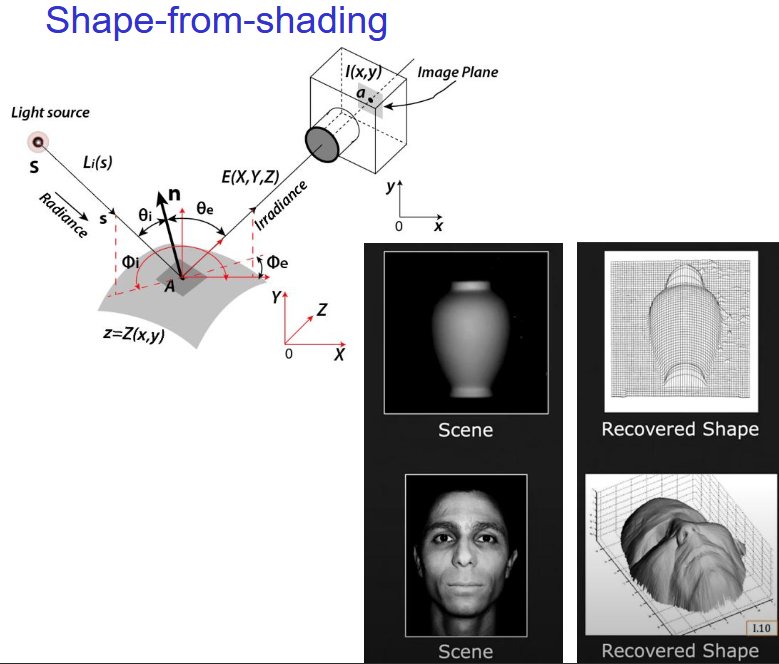
\includegraphics[width=0.5\linewidth,height=\textheight,keepaspectratio,alt={Shape from shading}]{image-60.png}
\caption{Shape from shading}
\end{figure}

\subsubsection{Multi-directional}\label{multi-directional}

\paragraph{Basic Stereo vision}\label{basic-stereo-vision}

The idea is to use triangulation like we do with our eyes. By using two
cameras with a known baseline, we can find the depth of the scene by
looking at the disparity between the two images. The disparity is the
difference in the position of the same point in the two images

\begin{figure}
\centering
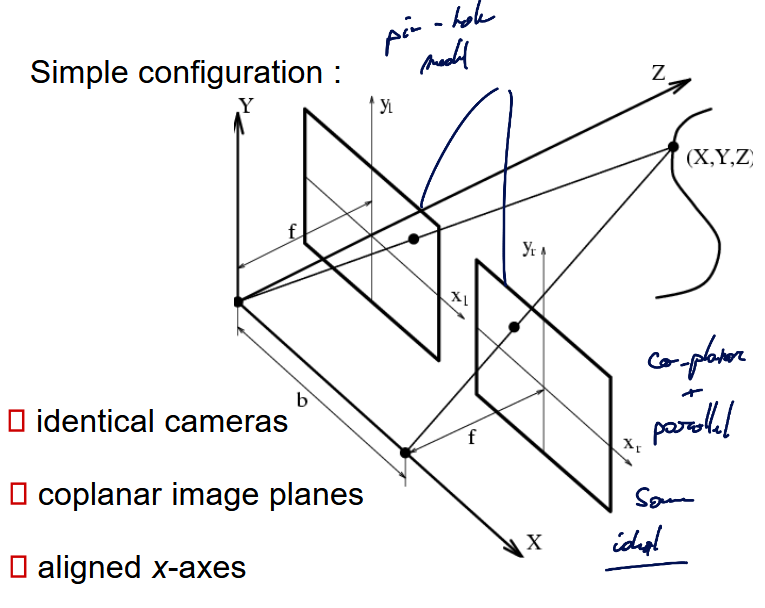
\includegraphics[width=0.5\linewidth,height=\textheight,keepaspectratio,alt={Passive stereo}]{image-61.png}
\caption{Passive stereo}
\end{figure}

With this basic setup, the object will lie on the saame scanline in both
images but the vertical line will be somewhat different. Remember the
camera projection with the \(K\) camera calbration matrix, \(R\) the
rotation matrix, \(P\) the 3D point and \(C\) the camera center:

\[
\rho p = K R^\top (P-C)
\]

If we ``attach'' the world coordinate to the left camera, we can remove
\(R\) since \(=I\) and \(C=0\). With a distance \(b\) separating the two
cameras and by normalizing the focal length to 1, we can find the depth
\(Z\) of the point in the scene with:

\[
\rho \begin{pmatrix}
    x\\
    y\\
    1
\end{pmatrix} = K \begin{pmatrix}
    X\\
    Y\\
    Z
\end{pmatrix} \qquad \rho \begin{pmatrix}
    x'\\
    y'\\
    1
\end{pmatrix} = K \begin{pmatrix}
    X-b\\
    Y\\
    Z
\end{pmatrix} \qquad K = \begin{matrix}
    fk_x & 0 & 0\\
    0 & fk_y & 0\\
    0 & 0 & 1
\end{matrix} \qquad Z = \frac{fbk_x}{x-x'}
\]

\begin{equation}
\begin{cases}
    x = \frac{fk_x X}{Z}\\
    y = \frac{fk_y Y}{Z}
    
\end{cases} \qquad \begin{cases}
    x' = \frac{fk_x (X-b)}{Z}\\
    y' = \frac{fk_y Y}{Z}
\end{cases}
\end{equation}

\(k_x\) is required for non-square pixels which is 1/horizontal pixel
size and \(k_y\) is 1/vertical pixel size. \(k_x=k_y=1\) for square
pixels. The depth is inversely proportional to the disparity \(x-x'\).
The larger the disparity, the closer the object is to the camera. The
smaller the disparity, the farther the object is from the camera.

When observing the same points in two view, using the \textbf{disparity}
\((x-x')\), imprecise for far away objects (increase b or f to improve
accuracy, but it reduces the simultaneous visibility) we have:

\[
X = b \frac{x}{(x-x')} \qquad Y = b \frac{k_x}{k_y} \frac{y}{(x-x')} \qquad Z = b k_x \frac{f}{(x-x')}
\]

Huan stereo vision is good only up to \(\pm10\) meters, the human brain
will use experience to infer distance for the rest. The real issue is
finding the two right correspondances (almoss impossible for untextured
objects).

\paragraph{General Stereo vision}\label{general-stereo-vision}

\begin{figure}
\centering
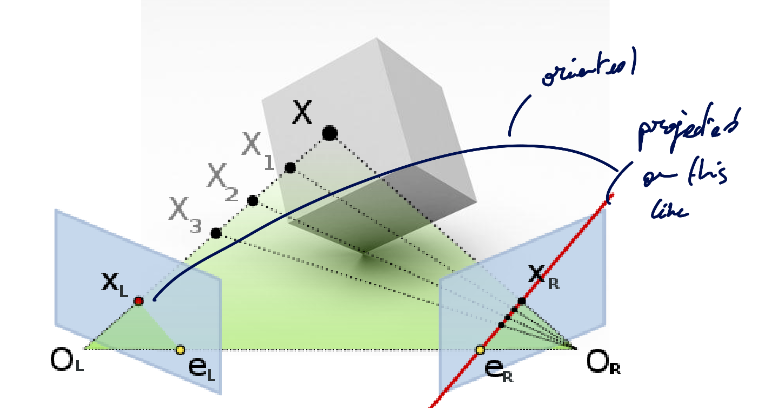
\includegraphics[width=0.5\linewidth,height=\textheight,keepaspectratio,alt={General setup}]{image-63.png}
\caption{General setup}
\end{figure}

Now, the planes are not necessarily parallel and the cameras are not
necessarily on the same plane. We can use the epipolar geometry to find
the correspondance between the two images. The idea is to find the
epipolar lines in both images and then look for correspondance along
these lines. This is called the \textbf{epipolar constraint}. The
epipolar constraint states that the point in one image must lie on the
epipolar line in the other image. We can then use the disparity along
the epipolar line to find the depth of the scene. This method requires
both camera to be properly calibrated and the relative position,
orientation, and setting of the cameras to be known.

\[
\mu p = KR^\top (P-C) \qquad \rho' p' = KR'^\top (P-C') \qquad \text{the Ray: } P = C+\mu RK^{-1}p \quad \mu \in \mathbb{R}
\]

Not be studied but good for understanding. The point \(P\) must lie on
the ray defined by the camera center and the point in the image. We can
then find the epipolar line by finding the intersection of the ray with
the image plane of the other camera using the equation
\(\rho' p' = KR'^\top (P-C')\). This is given by:

\[
\rho' p' = KR'^\top (C+\mu RK^{-1}p - C') \qquad \rho' p' = \underbrace{KR'^\top (C-C')}_{\text{Epipole}} + \underbrace{\mu KR'^\top RK^{-1}p}_{\text{Vanishing point}}
\]

The epipole is the point where the line connecting the two camera
centers intersects the image plane. The vanishing point is the point
where the ray defined by the camera center and the point in the image
intersects the image plane of the other camera. The epipolar line is
then given by the line connecting the epipole and the vanishing point.

We can then use the simplified notation with \(A\) the infinite
homography and \(e\) the epipole:

\[
A = \frac{1}{\rho'_e}K'R'^\top RK^{-1} \qquad e = \frac{1}{\rho'_e}KR'^\top (C-C') \qquad \rho' p' = \rho'_e (\mu A p + e')
\]

We can write the epipolar constraint as:

\[
|p'e'Ap| = p'^\top (e'\times Ap) = 0 \rightarrow |p'e'Ap| = p'^\top [e']_\times A p = 0 \quad \underbrace{F = [e']_\times A}_{\text{Fundamental matrix}} \quad [e']_\times = \begin{bmatrix}
    0 & -e'_z & e'_y\\
    e'_z & 0 & -e'_x\\
    -e'_y & e'_x & 0
\end{bmatrix}
\]

The fundamental matrix \(F\) encapsulates the epipolar geometry of the
two views. It is a 3x3 matrix which has rank 2. ( \(p'^\top F\) ) is a
triple (\(a',b',c'\)) giving the coefficients of the epipolar line for
point p with coordinates (\(x,y,1\)): \(a'\cdot x + b'\cdot y +c' = 0\).
And vice versa for \(Fp\).

\begin{figure}
\centering
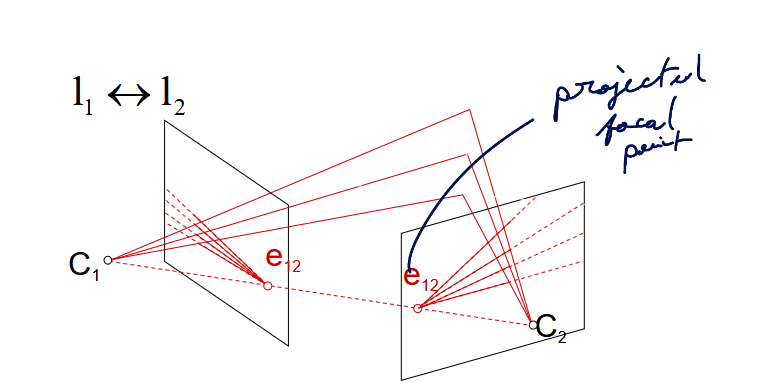
\includegraphics[width=0.5\linewidth,height=\textheight,keepaspectratio,alt={Epipolar lines are in mutual correspondance == allows to separate the matching problem}]{image-64.png}
\caption{Epipolar lines are in mutual correspondance == allows to
separate the matching problem}
\end{figure}

How to find the Fundamental matrix:

\begin{itemize}
\tightlist
\item
  One point yields one equation \(p'^\top F p = 0\) , that is linear in
  the entries of the fundamental matrix F so, we can actually obtain F
  without any prio knowledge about camera settings if we have sufficient
  pairs of corresponding points !!
\item
  F can be computed linearly from 8 pairs of corresponding points; not
  9, as this is a homogeneous system of equations.
\item
  F being rank 2 yileds an additional, but non-linear constraint (
  det(F)=0 ), thus 7 correspondences suffice to non-linearly solve for F
\end{itemize}

In practice,

\begin{itemize}
\tightlist
\item
  Detect interest points (using detector) that are good candidates to
  serve as initial correspondence sand match features
  (e.g.~SIFT/ORB/etc.)
\item
  Solve the 8-point algorithm using e.g.~least squares and find the
  point pairs that fit the model using RANSAC (this is to avoid false
  positives, RANSAC randomly selects initial pairs, and adds pairs
  gradually while the F-equation remains between bounds)
\item
  Estimate final F (this might not have rank 2, because of noise,
  imperfect matches, measurement errors rank will almost always by
  full=3)
\item
  Enforce rank 2 using SVD: decompose \(F=U\Sigma VT\), singular values
  are in \(\Sigma=diag(\sigma_1,\sigma_2,\sigma_3)\), and force
  \(\sigma_3=0\).
\end{itemize}

Epipolar lines are in mutual correspondence. Separate 2D correspondence
search problem to 1D search problem by using two view geometry

We can also reduce the search space by only picking points on the
epipolar line, min and max depth for line segmaet, smoothness of the
disparity field, \ldots{}

Again this is for reference and the math derivation presented here is
not required for the exam, but it is good to understand the underlying
principles of stereo vision and epipolar geometry. By re-using the ray
equation and epipolar constraint we have 6equations and 5 unknowns (over
determined set of equations). Siometimes the ray may not interesect due
to noise so we take the middle.

\[
P = C+\mu RK^{-1}p \quad \mu \in \mathbb{R} \qquad P = C'+\mu' R'K'^{-1}p' \quad \mu' \in \mathbb{R}
\]

\paragraph{Multiview stereo}\label{multiview-stereo}

We can expand this idea to multi-view stereo where we have a moving
camera and we want to reconstruct the 3D scene from multiple images. We
can use the same principles as stereo vision but we need to take into
account the motion of the camera. We can use structure from motion (SfM)
to find the camera motion and then use multi-view stereo to reconstruct
the 3D scene.

We must do feature tracking, estimate pairwise geometry, and then do
multi-view stereo to reconstruct the 3D scene. This is a complex process
but it allows us to reconstruct the 3D scene from multiple images. We
must also self-calibrate to understand the intrinsic parameters of the
camera \(K\) and the relative position and orientation of the cameras.
Convert it to another base \(E=K^\top FK\).

\subsection{Active: interere with the scene to get
information}\label{active-interere-with-the-scene-to-get-information}

\subsubsection{Uni-directional}\label{uni-directional-1}

\paragraph{Time-of-flight}\label{time-of-flight}

This is the idea behind radar or lidar, we measure the time-of-flight of
a pulse or we analyze the phase shift of a continuous wave to find the
distance of the object. It is a direct way to measure depth but it can
be affected by noise, multipath interference, and other factors. We can
cast multiple ray to get a point cloud of the scene. The distance is
given by:

\[
d = \frac{c \cdot t}{2} \qquad d = \frac{c \cdot \phi}{4\pi f}
\]

\subsubsection{Multi-directional}\label{multi-directional-1}

\paragraph{Line scanning}\label{line-scanning}

The idea is to simplify the stereo vision by projecting a line on the
scene and then looking at the deformation of the line to infer the 3D
structure of the scene. This is a simple but effective way to
reconstruct the 3D scene. It is often used in industrial applications
for quality control and inspection. We can cast a cloud of points and
capture the deformation of the line to reconstruct the 3D scene. It is a
direct way to measure depth but it can be affected by noise, occlusion,
and other factors and find no interesection points !.

\begin{figure}
\centering
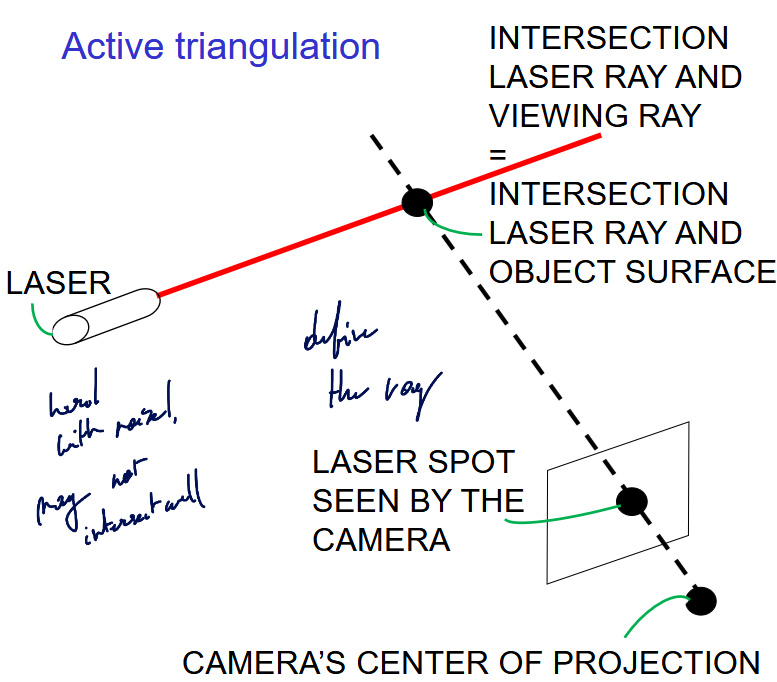
\includegraphics[width=0.5\linewidth,height=\textheight,keepaspectratio,alt={Active triangulation}]{image-66.png}
\caption{Active triangulation}
\end{figure}

\begin{figure}
\centering
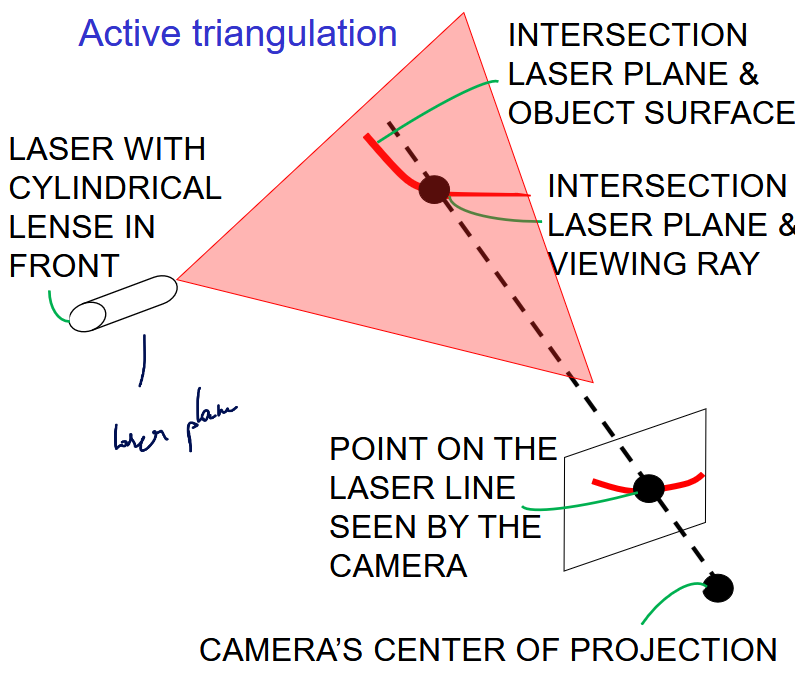
\includegraphics[width=0.5\linewidth,height=\textheight,keepaspectratio,alt={Active triangluation: with a plane, noise has less influence}]{image-67.png}
\caption{Active triangluation: with a plane, noise has less influence}
\end{figure}

\paragraph{Structured light}\label{structured-light}

The idea is to project a pattern of light on the scene and then look at
the deformation of the pattern to infer the 3D structure of the scene.
The goal is to have minimum number of pattern projection while keeping a
good resolution. For example, we can use serial binary patterns with
incresingly fine subdivisions \(2^n\). Or we can use colors \(3^n\).
Finally we can use a checkerboard pattern with a column code giving one
shot implementation. The kinect uses \(9\times 9\) with unique code.

\begin{figure}
\centering
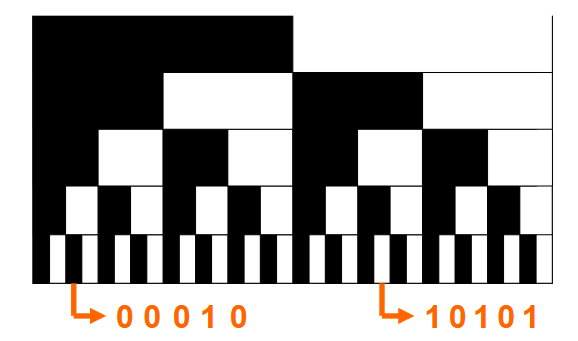
\includegraphics[width=0.5\linewidth,height=\textheight,keepaspectratio,alt={Serial binary patterns}]{image-68.png}
\caption{Serial binary patterns}
\end{figure}

\paragraph{Photometric stereo}\label{photometric-stereo}

Again based on the lambertian assumption, we will change the light
actively to observe the object under various lighting conditions. Can
give really high contrast and depth for small objects with little
texture.

\newpage
\part{Modern Image Analysis}

\begin{longtable}[]{@{}
  >{\raggedright\arraybackslash}p{(\linewidth - 4\tabcolsep) * \real{0.0524}}
  >{\raggedright\arraybackslash}p{(\linewidth - 4\tabcolsep) * \real{0.0175}}
  >{\raggedright\arraybackslash}p{(\linewidth - 4\tabcolsep) * \real{0.9301}}@{}}
\caption{Summary of notorious DeepLearning network}\tabularnewline
\toprule\noalign{}
\begin{minipage}[b]{\linewidth}\raggedright
Network name
\end{minipage} & \begin{minipage}[b]{\linewidth}\raggedright
Type
\end{minipage} & \begin{minipage}[b]{\linewidth}\raggedright
Characteristics
\end{minipage} \\
\midrule\noalign{}
\endfirsthead
\toprule\noalign{}
\begin{minipage}[b]{\linewidth}\raggedright
Network name
\end{minipage} & \begin{minipage}[b]{\linewidth}\raggedright
Type
\end{minipage} & \begin{minipage}[b]{\linewidth}\raggedright
Characteristics
\end{minipage} \\
\midrule\noalign{}
\endhead
\bottomrule\noalign{}
\endlastfoot
Alexnet & CNN & 8 layers, 60 million parameters, 1.2 million images,
1000 classes; handcrafted sizes \\
VGGNet & CNN & 19 layers, 138 million parameters, 1.2 million images,
1000 classes; use 3x3 CNN, when pooling double depth if we divide height
and width by 2, more mature. Declined in model sizes VGG-XX with XX
layers. \\
ResNet & CNN & 152 layers, 25 million parameters, 1.2 million images,
1000 classes; use residual connections to avoid vanishing gradient
problem, more mature. Declined in model sizes ResNet-XX with XX layers.
Use average pooling \\
\end{longtable}

\begin{figure}
\centering
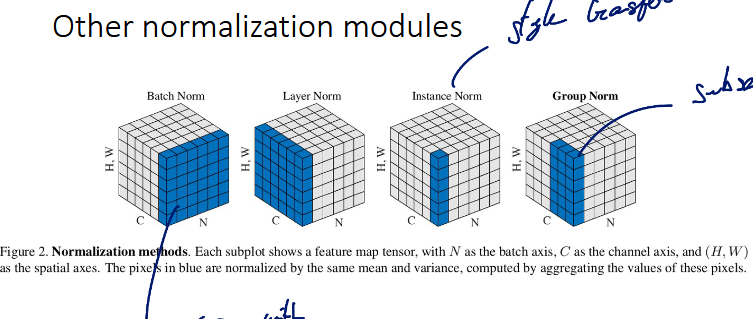
\includegraphics[width=0.7\linewidth,height=\textheight,keepaspectratio,alt={Type of normalization; N is the batch size, C are the channels, HxW are the spatial dimensions}]{image-69.png}
\caption{Type of normalization; N is the batch size, C are the channels,
HxW are the spatial dimensions}
\end{figure}

\begin{figure}
\centering
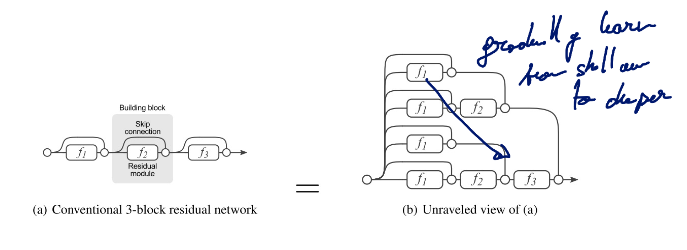
\includegraphics[width=0.7\linewidth,height=\textheight,keepaspectratio,alt={Resnet interpretation}]{image-70.png}
\caption{Resnet interpretation}
\end{figure}

\begin{figure}
\centering
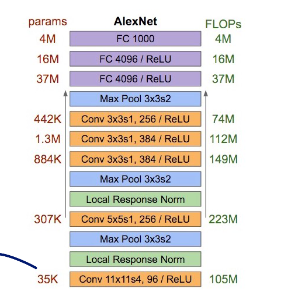
\includegraphics[width=0.3\linewidth,height=\textheight,keepaspectratio,alt={Size estimation for a CNN and its head}]{image-72.png}
\caption{Size estimation for a CNN and its head}
\end{figure}

\begin{figure}
\centering
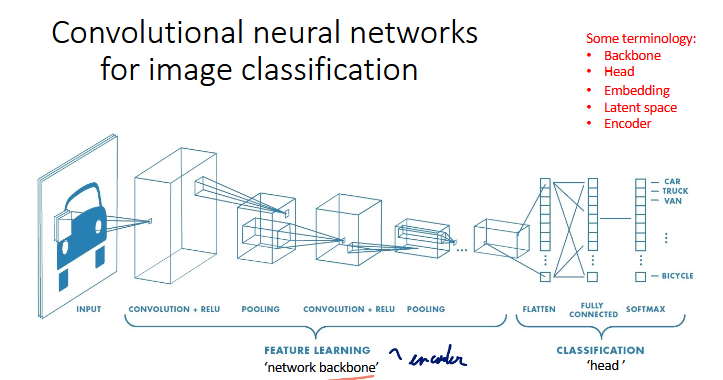
\includegraphics[width=0.7\linewidth,height=\textheight,keepaspectratio,alt={Typical CNN and its nomenclature}]{image-71.png}
\caption{Typical CNN and its nomenclature}
\end{figure}

\begin{longtable}[]{@{}
  >{\raggedright\arraybackslash}p{(\linewidth - 4\tabcolsep) * \real{0.2632}}
  >{\raggedright\arraybackslash}p{(\linewidth - 4\tabcolsep) * \real{0.2180}}
  >{\raggedright\arraybackslash}p{(\linewidth - 4\tabcolsep) * \real{0.5188}}@{}}
\caption{Loss function and use case}\tabularnewline
\toprule\noalign{}
\begin{minipage}[b]{\linewidth}\raggedright
Type of loss
\end{minipage} & \begin{minipage}[b]{\linewidth}\raggedright
Usecase
\end{minipage} & \begin{minipage}[b]{\linewidth}\raggedright
Math
\end{minipage} \\
\midrule\noalign{}
\endfirsthead
\toprule\noalign{}
\begin{minipage}[b]{\linewidth}\raggedright
Type of loss
\end{minipage} & \begin{minipage}[b]{\linewidth}\raggedright
Usecase
\end{minipage} & \begin{minipage}[b]{\linewidth}\raggedright
Math
\end{minipage} \\
\midrule\noalign{}
\endhead
\bottomrule\noalign{}
\endlastfoot
softmax + Cross-entropy loss & Classification (1 class) &
\(L = -\sum_{i=1}^N y_i \log(\hat{y}_i)\) \\
Sigmoid + Binary Cross-entropy loss & Classification (multi-label) &
\(L = -\sum_{i=1}^N [y_i \log(\hat{y}_i) + (1-y_i) \log(1-\hat{y}_i)]\) \\
L1,L2,Huber loss & Regression (continuous value) & \$L =\sum\_\{i=1\}\^{}N$ \\
\end{longtable}

\begin{longtable}[]{@{}
  >{\raggedright\arraybackslash}p{(\linewidth - 4\tabcolsep) * \real{0.0396}}
  >{\raggedright\arraybackslash}p{(\linewidth - 4\tabcolsep) * \real{0.0231}}
  >{\raggedright\arraybackslash}p{(\linewidth - 4\tabcolsep) * \real{0.9373}}@{}}
\caption{Object detection NN}\tabularnewline
\toprule\noalign{}
\begin{minipage}[b]{\linewidth}\raggedright
Name of NN
\end{minipage} & \begin{minipage}[b]{\linewidth}\raggedright
Type
\end{minipage} & \begin{minipage}[b]{\linewidth}\raggedright
Characteristics
\end{minipage} \\
\midrule\noalign{}
\endfirsthead
\toprule\noalign{}
\begin{minipage}[b]{\linewidth}\raggedright
Name of NN
\end{minipage} & \begin{minipage}[b]{\linewidth}\raggedright
Type
\end{minipage} & \begin{minipage}[b]{\linewidth}\raggedright
Characteristics
\end{minipage} \\
\midrule\noalign{}
\endhead
\bottomrule\noalign{}
\endlastfoot
R-CNN & 2-stage & Region-based CNN, uses selective search to find region
proposals and then applies a CNN to each proposal to classify it. Use
SVM classification --\textgreater{} no end-to-end training \\
Fast R-CNN & 2-stage & An improvement over R-CNN, it uses a single CNN
to extract features from the entire image and then applies a region of
interest (RoI) pooling layer to classify each proposal. Use a linear
classifier (Cross-entropy for label classification and Huber Loss for
regression (bounding box)) \\
Faster R-CNN & 2-stage & An improvement over Fast R-CNN, it uses a
region proposal network (RPN) to generate region proposals instead of
selective search, making it faster and more efficient. \\
Mask R-CNN & 2-stage & An improvement over Faster R-CNN, it adds a
branch for predicting segmentation masks on each region of interest, in
addition to the existing branches for classification and bounding box
regression. \\
YOLO & 1-stage & You Only Look Once, it divides the image into a grid
and predicts bounding boxes and class probabilities for each grid cell,
making it faster but less accurate than 2-stage methods. \\
\end{longtable}

\begin{figure}
\centering
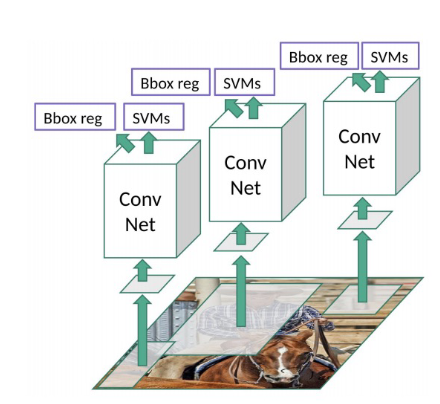
\includegraphics[width=0.5\linewidth,height=\textheight,keepaspectratio,alt={R-CNN}]{image-73.png}
\caption{R-CNN}
\end{figure}

\begin{figure}
\centering
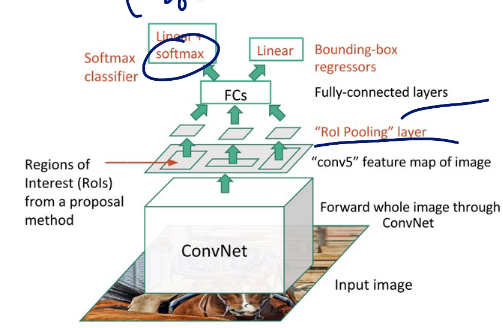
\includegraphics[width=0.5\linewidth,height=\textheight,keepaspectratio,alt={Fast R-CNN}]{image-74.png}
\caption{Fast R-CNN}
\end{figure}

\begin{figure}
\centering
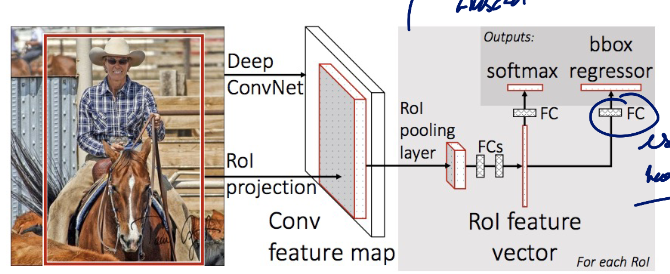
\includegraphics[width=0.5\linewidth,height=\textheight,keepaspectratio,alt={In-depth Fast R-CNN}]{image-75.png}
\caption{In-depth Fast R-CNN}
\end{figure}

\begin{figure}
\centering
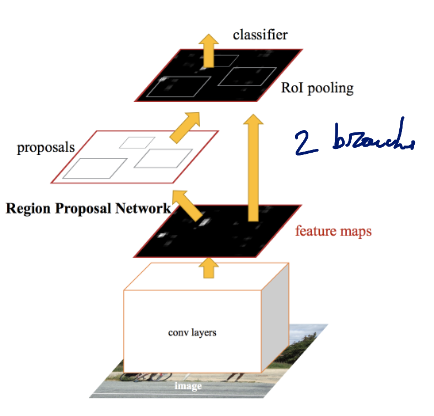
\includegraphics[width=0.5\linewidth,height=\textheight,keepaspectratio,alt={Faster R-CNN}]{image-76.png}
\caption{Faster R-CNN}
\end{figure}

\newpage

\section{License}\label{license}

This work is licensed under a
\href{https://creativecommons.org/licenses/by-nc-sa/4.0/}{Creative
Commons Attribution-NonCommercial-ShareAlike 4.0 International License
(CC BY-NC-SA 4.0)} for KU Leuven students.

You are free to:

\begin{itemize}
\tightlist
\item
  \textbf{Share} --- copy and redistribute the material in any medium or
  format with people inside of KU Leuven or being granted access to the
  source material.
\item
  \textbf{Adapt} --- remix, transform, and build upon the material if
  you are a KU Leuven student.
\end{itemize}

Under the following terms:

\begin{itemize}
\tightlist
\item
  \textbf{Attribution} --- You must give appropriate credit, provide a
  link to the license, and indicate if changes were made. You may do so
  in any reasonable manner, but not in any way that suggests the
  licensor endorses you or your use.
\item
  \textbf{NonCommercial} --- You may not use the material for commercial
  purposes.
\item
  \textbf{ShareAlike} --- If you remix, transform, or build upon the
  material, you must distribute your contributions under the same
  license as the original.
\end{itemize}

For the full legal text of the license, please visit:
\url{https://creativecommons.org/licenses/by-nc-sa/4.0/legalcode}

\subsection{Modification}\label{modification}

To contribute to this work or any other one from this project please
find more information at the
\href{https://github.com/Tfloow/ESATSummary}{Github repository}.

\subsection{Take down}\label{take-down}

If you are a professor or representing any official party and wish to
take down this work, you can submit a takedown request at this url:
\url{https://github.com/Tfloow/ESATSummary/issues/new?template=takedown_notice.yml}

\begin{center}\rule{0.5\linewidth}{0.5pt}\end{center}

\textbf{Some Rights Reserved \the\year{} Authors of the Summary,
Professors of the Course and possible book's authors. Some Rights
Reserved.}

\end{document}
